\documentclass[12pt]{article}
\usepackage{mathematics}

\begin{document}

\title{Oxford M2 - Real Analysis I - Sequences and Series
  \footnotetext{\url{https://courses.maths.ox.ac.uk/node/37482}}} \author{Dan Davison}
\author{}
\date{}
\maketitle

\section{Sheet 1}

\newpage
\subsection{}
\begin{mdframed}
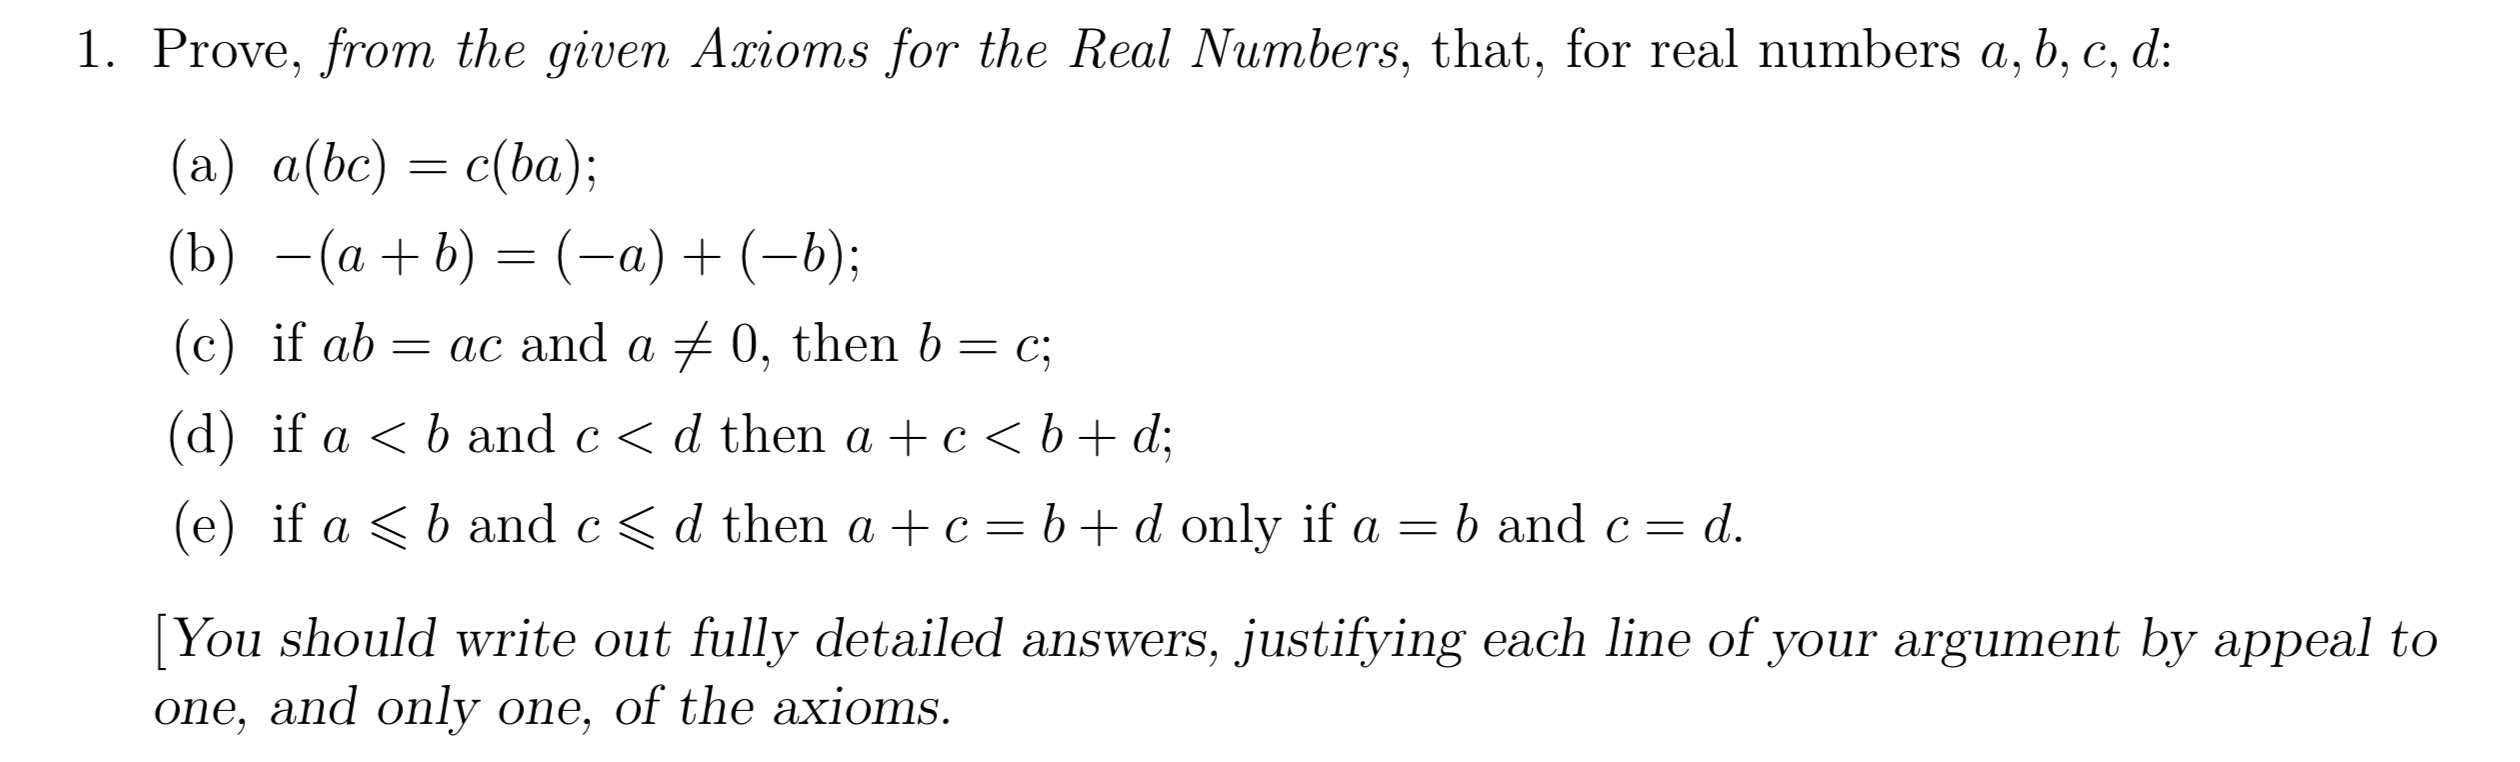
\includegraphics[width=400pt]{img/oxford-M2-analysis-I-1-1.png}
\end{mdframed}

\begin{enumerate}[label=(\alph*)]
\item \begin{claim*} $a(bc) = c(ba)$\end{claim*}
  \begin{proof}
    \begin{align*}
      a(bc) &= a(cb)  ~~~~~~~ \text{(M1 commutativity of multiplication)}\\
            &= (ac)b  ~~~~~~~ \text{(M2 associativity of multiplication)}\\
            &= (ca)b  ~~~~~~~ \text{(M1 commutativity of multiplication)}\\
            &= c(ab)  ~~~~~~~ \text{(M2 associativity of multiplication)}\\
            &= c(ba)  ~~~~~~~ \text{(M1 commutativity of multiplication)}
    \end{align*}
  \end{proof}
\newpage
\item
  \begin{claim*}
    $-(a + b) = (-a) + (-b)$
  \end{claim*}
  \begin{proof}
    \begin{align*}
      (a + b) + ((-a) + (-b)) &= (a + b) + ((-b) + (-a)) ~~~~~~~ \text{S1 commutativity of sum}\\
                              &=  a + (b + ((-b) + (-a))) ~~~~~~~ \text{S2 associativity of sum}\\
                              &=  a + ((b + (-b)) + (-a)) ~~~~~~~ \text{S2 associativity of sum}\\
                              &=  a + ((-a)) ~~~~~~~ \text{definition of negative}\\
                              &=  0 ~~~~~~~ \text{definition of negative}\\
    \end{align*}
    Therefore $(-a) + (-b)$ is an additive inverse of $a + b$, as claimed. The additive inverse is
    unique by definition.
  \end{proof}
\end{enumerate}

\newpage
\subsection{}
\begin{mdframed}
  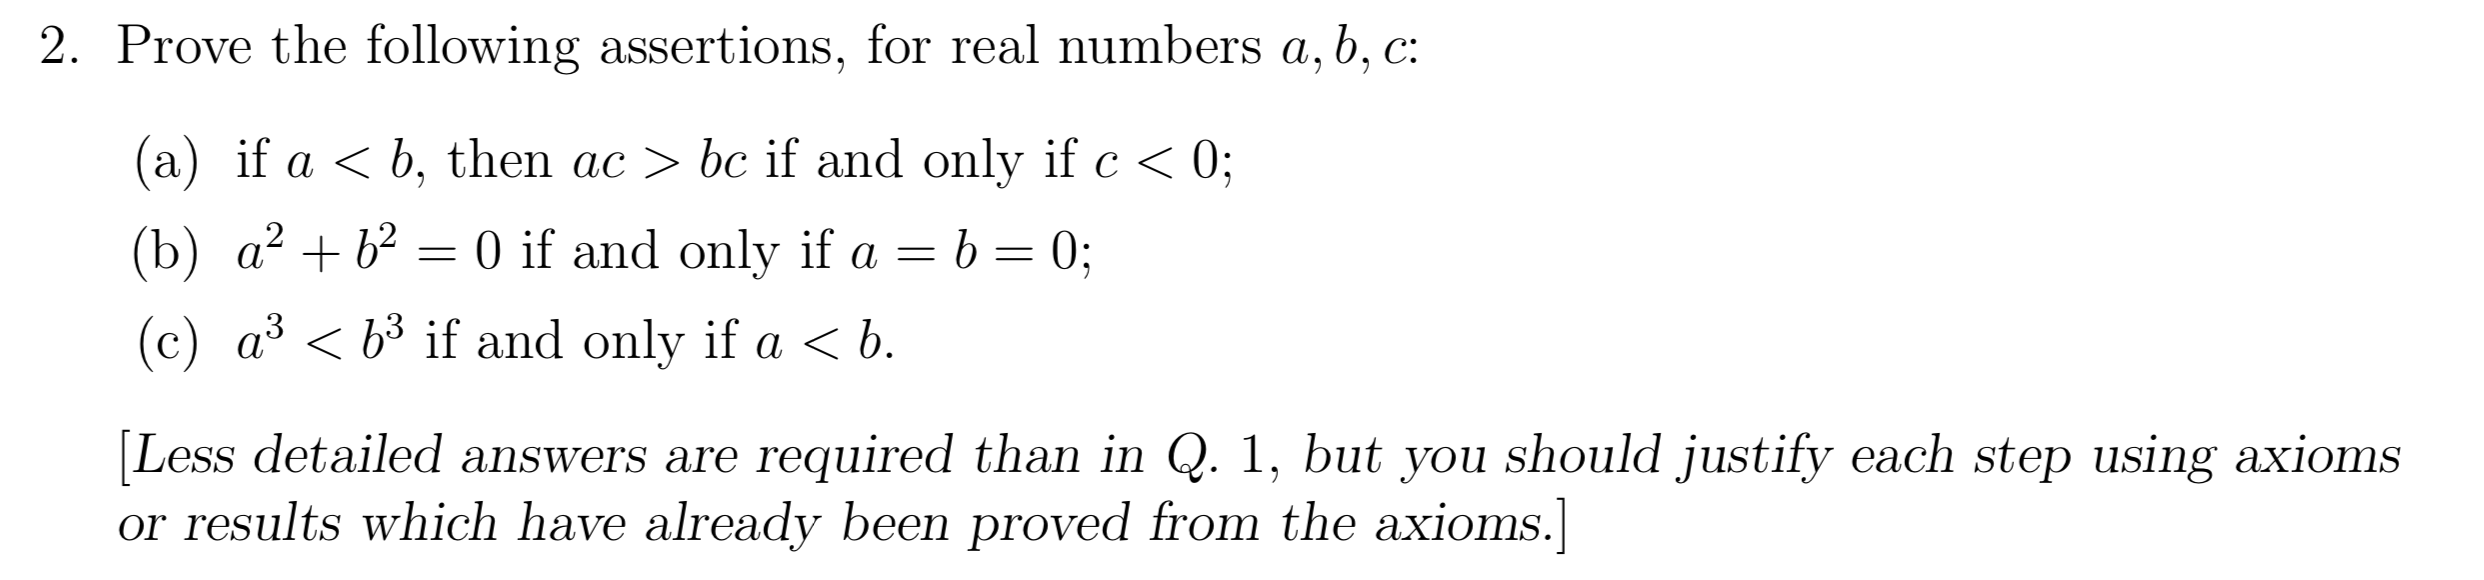
\includegraphics[width=400pt]{img/oxford-prelims-M2-analysis-I-sheet-1-2.png}
\end{mdframed}

\begin{enumerate}[label=(\alph*)]
\item
  \begin{claim*}
    If $a < b$ then $ac > bc$ iff $c < 0$.
  \end{claim*}
  \begin{intuition*}
    Multiplication by a scalar flips orientation iff the scalar is negative.
  \end{intuition*}
  \begin{proof}~\\
    \red{TODO} Prove carefully being explicit about which axioms are used.\\
    Let $\P$ be the strictly positive reals. We have $a < b$, i.e. $b - a \in \P$.\\
    $\implies$:\\
    We have $ac > bc$ i.e. $ac - bc \in \P$.

    Therefore
    \begin{align*}
      (a - b)c &\in \P\\
      (b - a)(-c) &\in \P\\
      \frac{1}{b-a}(b - a)(-c) &\in \P\\
      (-c) &\in \P
    \end{align*}

    $\impliedby$:\\
    We have $c < 0$, i.e. $-c \in \P$. Therefore $(-c)(b - a) \in \P$ (by {\bf P2}). Therefore
    $ac - bc \in \P$, i.e. $ac > bc$.
  \end{proof}
\end{enumerate}~\\

\newpage
\subsection{}
\begin{mdframed}
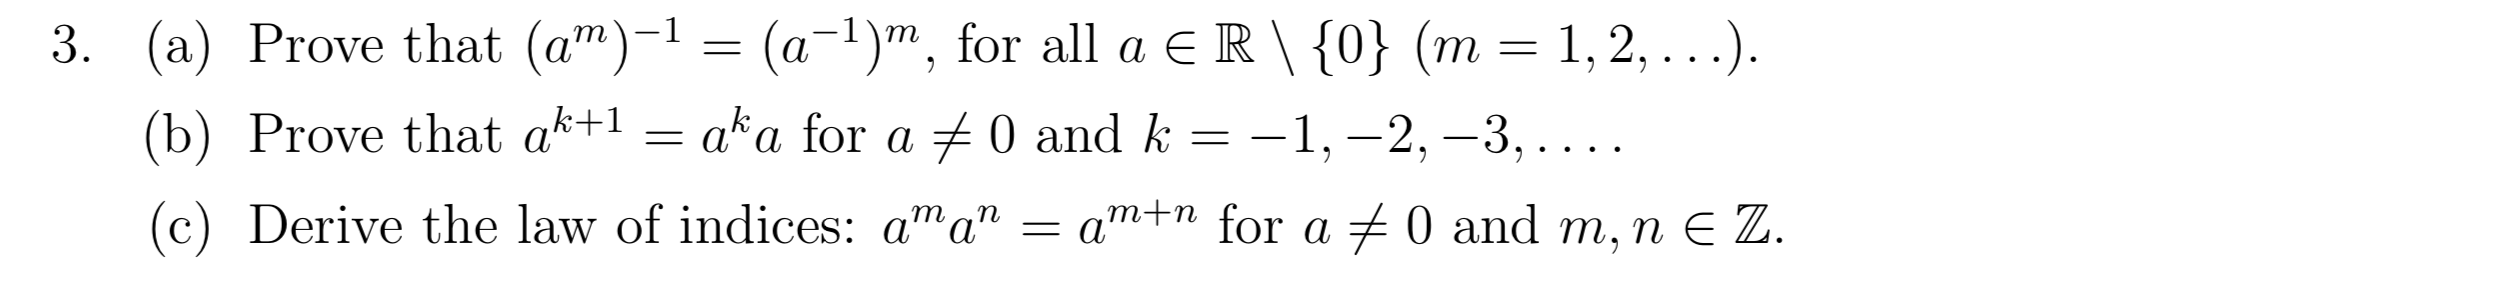
\includegraphics[width=400pt]{img/oxford-prelims-M2-analysis-I-sheet-1-3.png}
\end{mdframed}
\newpage
\subsection{}
\begin{mdframed}
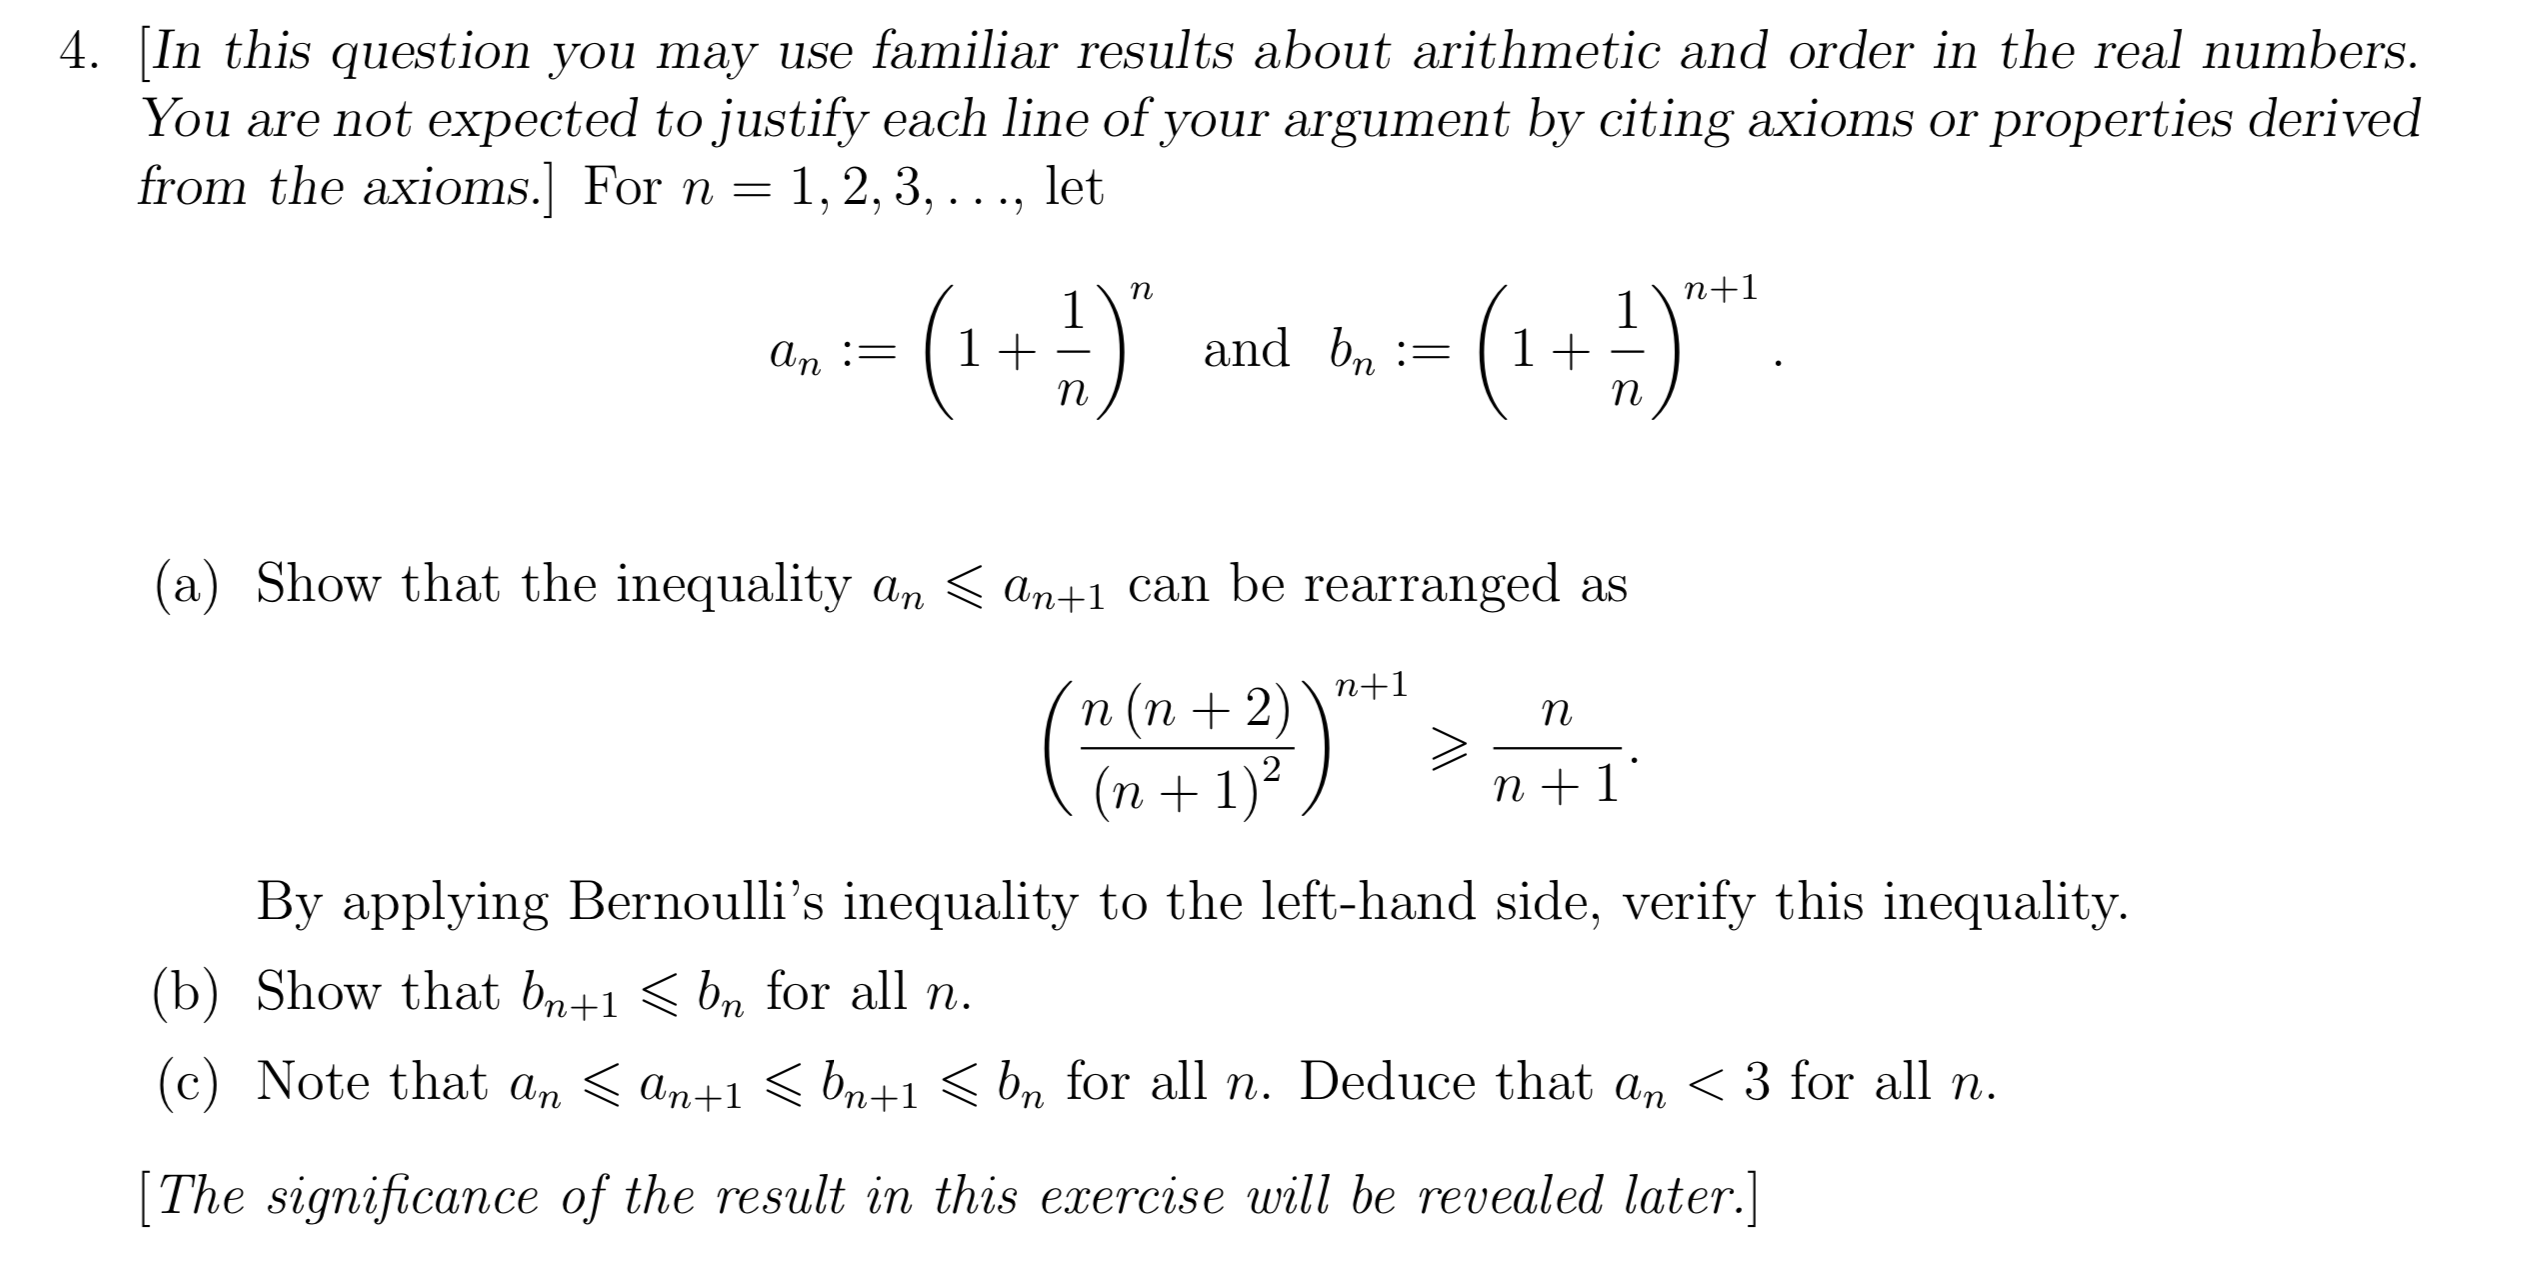
\includegraphics[width=400pt]{img/oxford-prelims-M2-analysis-I-sheet-1-4.png}
\end{mdframed}

\newpage
\subsection{}
\begin{mdframed}
  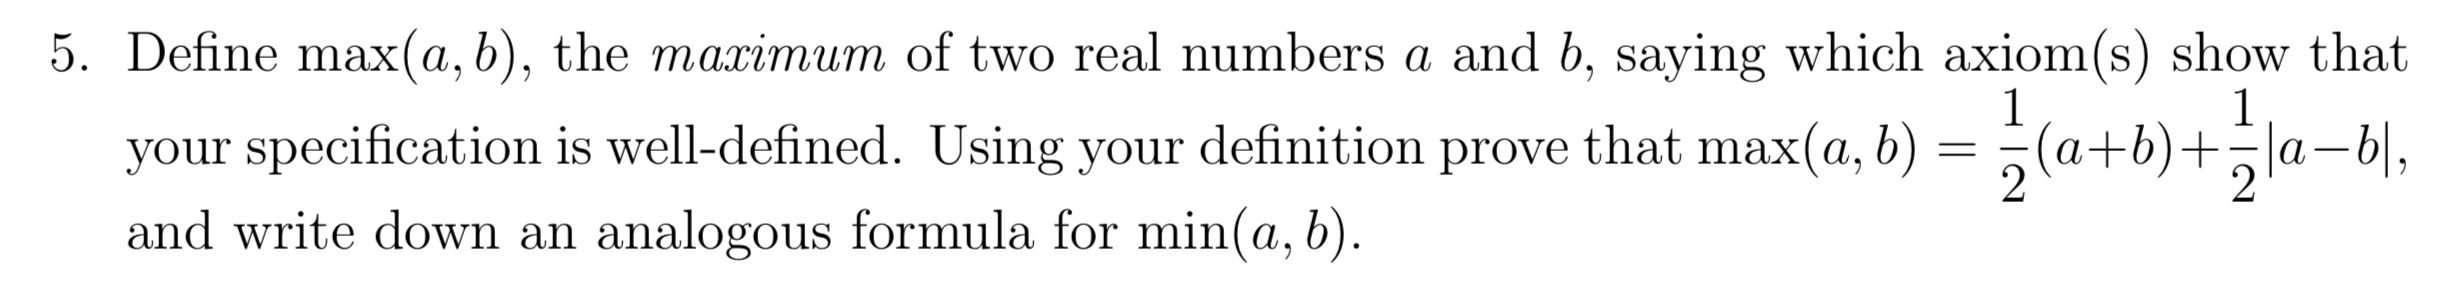
\includegraphics[width=400pt]{img/oxford-M2-analysis-I-1-5.png}
\end{mdframed}

\begin{definition*}
  Let $a, b \in \R$ with $a \neq b$.
  \begin{align*}
    \max(a, b) =
    \begin{cases}
      b ~~~~~~~&\text{if $a < b$}\\
      a ~~~~~~~&\text{if $b \leq a$}.
    \end{cases}
  \end{align*}
  This is well-defined by trichotomy of the order relation ($\max(a, b)$ has a unique value for
  alll $a, b \in \R$ since either $a < b$ or $a = b$ or $a > b$).
\end{definition*}

\begin{claim*}
  \begin{align*}
    \max(a, b) = \frac{1}{2}(a + b) + \frac{1}{2}|a - b|.
  \end{align*}
\end{claim*}

\begin{proof}
  Suppose $a = b$. Then
  \begin{align*}
    \frac{1}{2}(a + b) + \frac{1}{2}|a - b|
    = \frac{1}{2}\cdot 2a + \frac{1}{2}\cdot 0
    = a
    = \max(a, b).
  \end{align*}
  Since $(a + b) = (b + a)$ and $|a - b| = |b - a|$, we need only consider $a < b$ as the remaining
  alternative. Then $|a - b| = b - a$ and
  \begin{align*}
    \frac{1}{2}(a + b) + \frac{1}{2}|a - b|
    = \frac{1}{2}(a + b) + \frac{1}{2}(b - a)
    = b
    = \max(a, b).
  \end{align*}
\end{proof}

\newpage
\section{Sheet 2}

\newpage
\subsection{}
\begin{mdframed}
  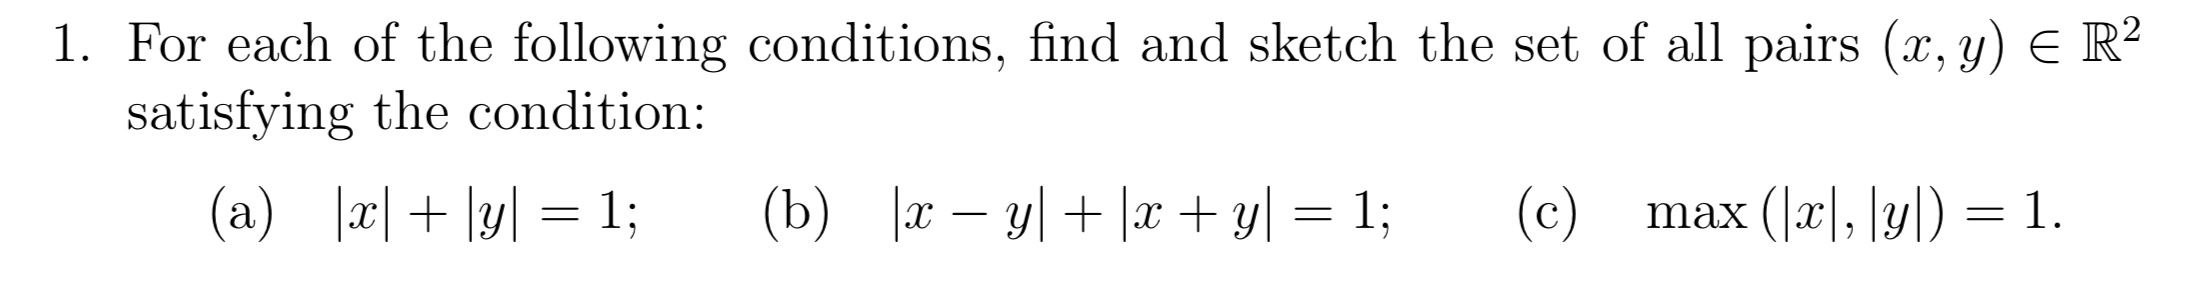
\includegraphics[width=400pt]{img/oxford-M2-analysis-I-2-1.png}
\end{mdframed}

\newpage
\subsection{}
\begin{mdframed}
  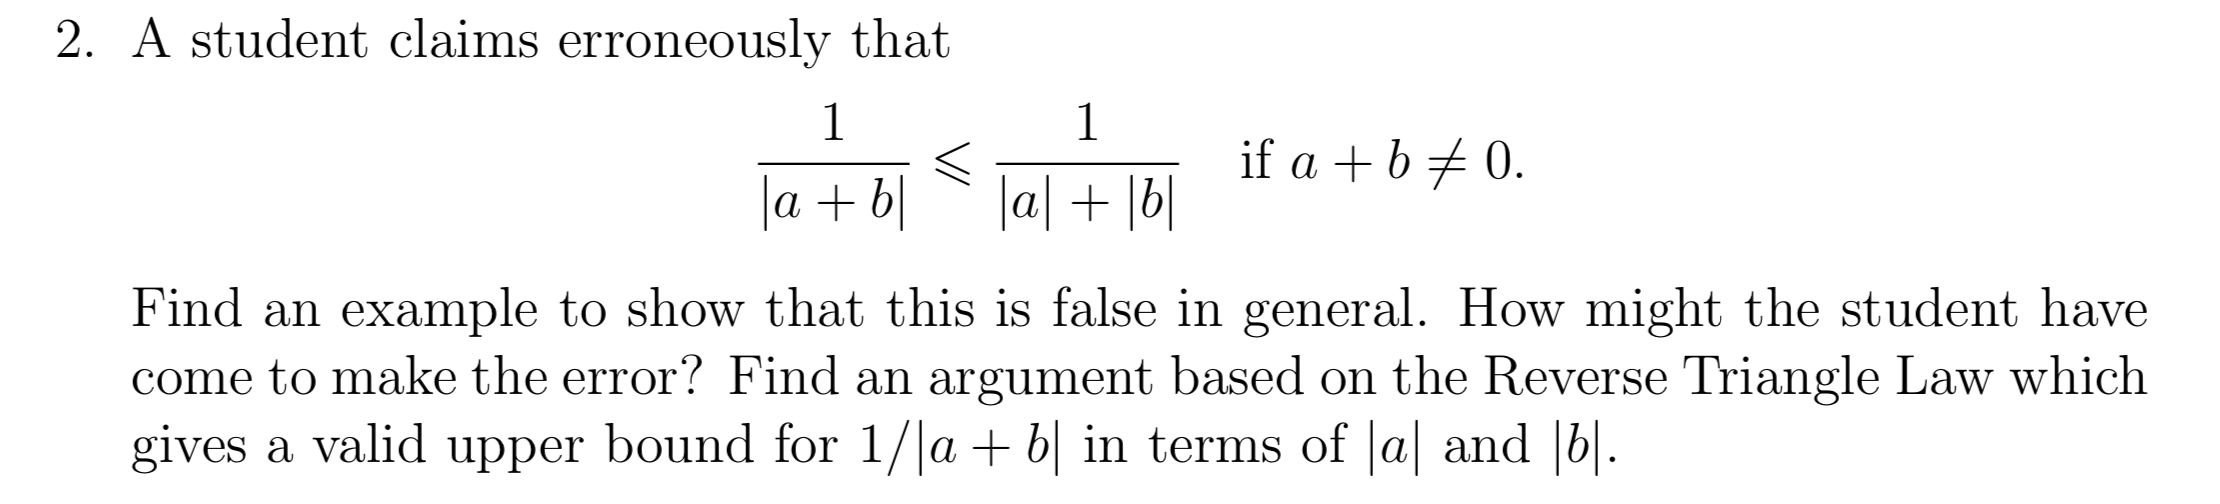
\includegraphics[width=400pt]{img/oxford-M2-analysis-I-2-2.png}
\end{mdframed}

\newpage
\subsection{(COMPLETE)}
\begin{mdframed}
  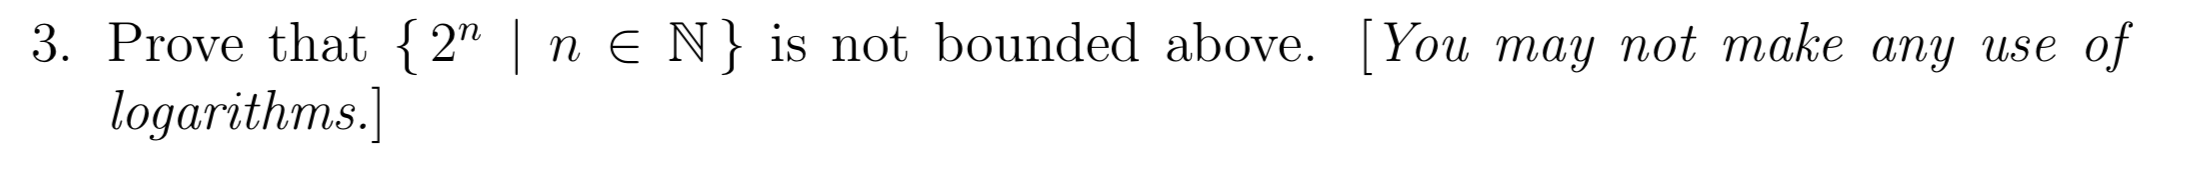
\includegraphics[width=400pt]{img/oxford-M2-analysis-I-2-3.png}
\end{mdframed}

\begin{proof}
  Let $S = \{2^n ~|~ n \in \N\}$ and suppose an upper bound for $S$ exists.

  Then $\sup S$ exists by completeness of the reals.

  By the Approximation Property there exists $2^k \in S$ such that
  \begin{align*}
    \sup S - \frac{1}{2} < 2^k \leq \sup S.
  \end{align*}
  Note that $k+1 \in \N$ therefore $2^{k+1} = 2^k + 2^k \in S$. Therefore
  \begin{align*}
    \sup S - \frac{1}{2} + 2^k &< 2^{k+1} \leq \sup S\\
    \sup S &\leq \sup S + \frac{1}{2} - 2^k < \sup S,
  \end{align*}
  a contradiction. Therefore no upper bound for $S$ exists.
\end{proof}

\newpage
\subsection{(COMPLETE)}
\begin{mdframed}
  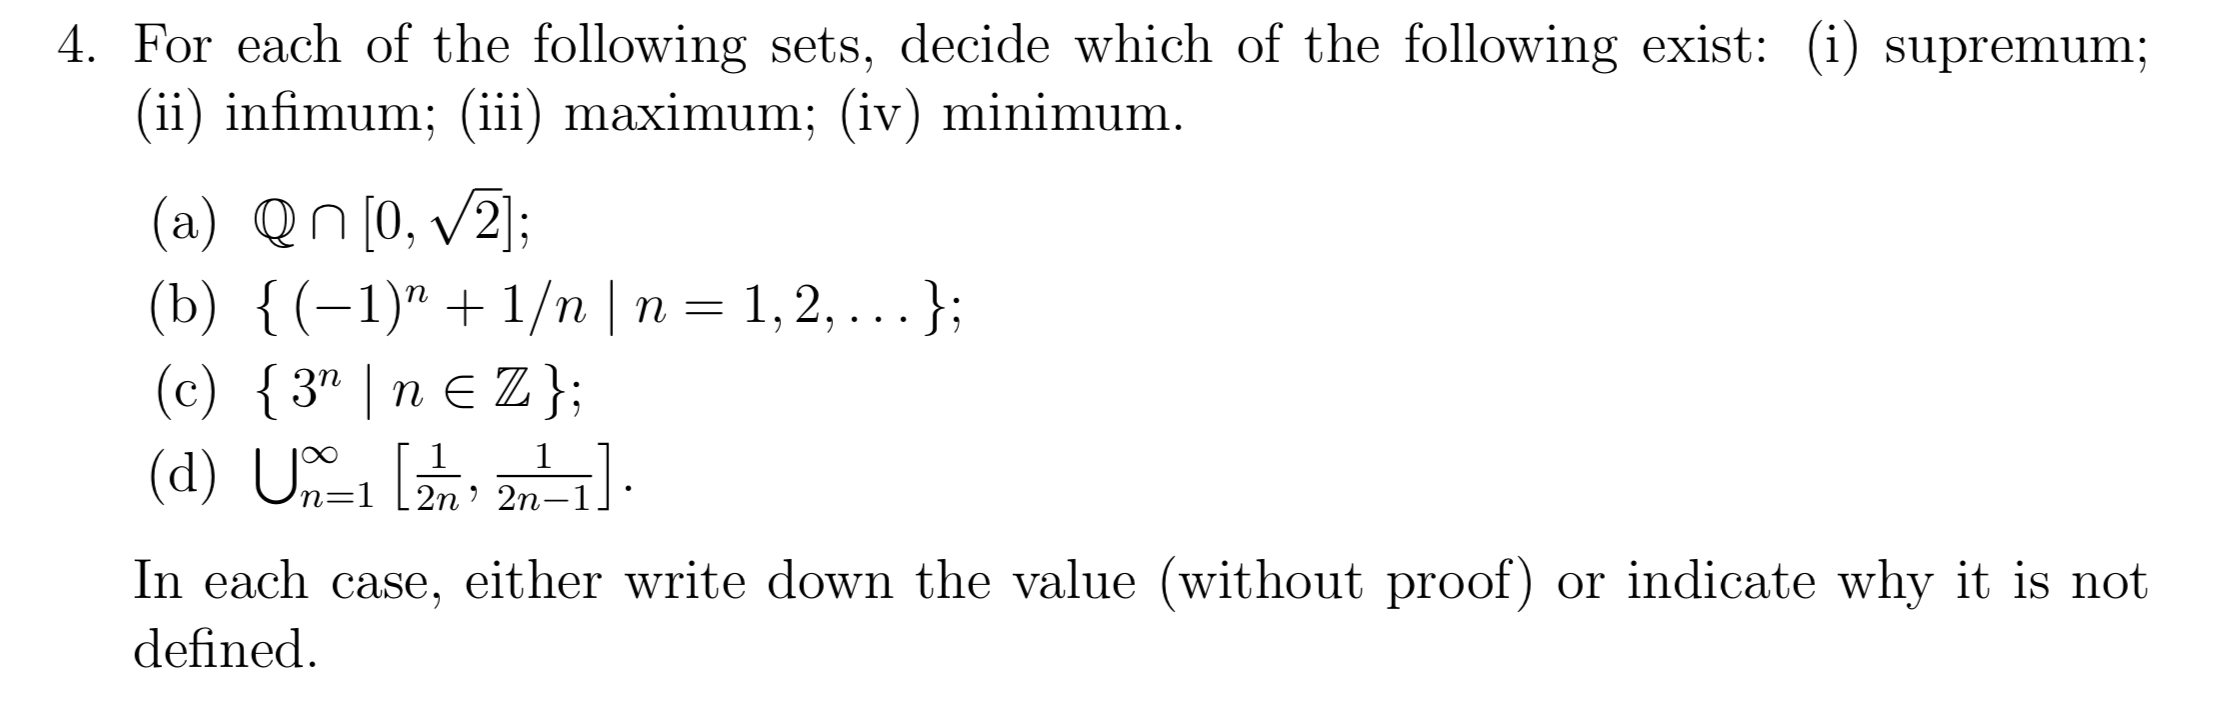
\includegraphics[width=400pt]{img/oxford-M2-analysis-I-2-4.png}
\end{mdframed}
\begin{enumerate}
\item $S = \Q \cap [0, \sqrt 2]$
  \begin{align*}
    \sup S &= \sqrt 2\\
    \max S &= \sqrt 2\\
    \min S &= 0\\
    \inf S &= 0
  \end{align*}
\item $S = \{(-1)^n + 1/n ~|~ n=1,2,\ldots\}$
  \begin{align*}
    \sup S &= 3/2\\
    \max S &= 3/2\\
    \min S ~&\text{does not exist since $\inf S \not\in S$}\\
    \inf S &= -1
  \end{align*}
\item $S = \{3^n ~|~ n \in \Z\}$
  \begin{align*}
    \sup S ~&\text{does not exist, $S$ has no upper bound}\\
    \max S ~&\text{does not exist, $S$ has no upper bound}\\
    \min S ~&\text{does not exist, $S$ has no lower bound}\\
    \inf S &= 0
  \end{align*}
\item $S = \cup_{n=1}^\infty [\frac{1}{2n}, \frac{1}{2n - 1}]$
  \begin{align*}
    \sup S ~&= 1\\
    \max S ~&= 1\\
    \min S ~&\text{does not exist, $S$ has no lower bound}\\
    \inf S ~&=0
  \end{align*}
\end{enumerate}

\newpage
\subsection{(COMPLETE)}
\begin{mdframed}
  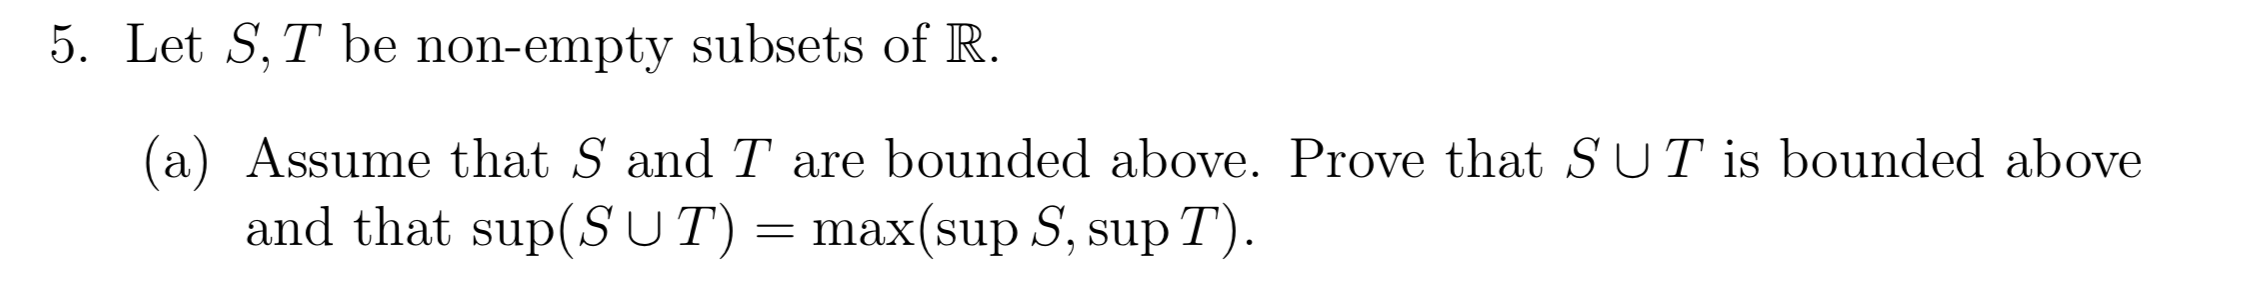
\includegraphics[width=400pt]{img/oxford-M2-analysis-I-2-5-a.png}
\end{mdframed}

\begin{proof}
  Let $S, T \subset \R$ with $S, T \neq \emptyset$. Assume that $S$ and $T$ are bounded
  above. Then $\sup S$ and $\sup T$ exist. Let $b = \max(\sup S, \sup T)$.

  Then $b \geq s$ for all $s \in S$ and $b \geq t$ for all $t \in T$. Therefore $b$ is an upper
  bound for $S \cup T$.

  Suppose there exists $a < b$ such that $a$ is an upper bound of $S \cup T$. Then either
  $a < \sup S$ or $a < \sup T$. Without loss of generality, suppose $a < \sup S$. Then $a$ is not
  an upper bound of $S$. Therefore there exists $s \in S$ such that $s > a$. But
  $s \in S \cup T$, therefore $a$ is not an upper bound of $S \cup T$, a contradiction.
\end{proof}

\begin{mdframed}
  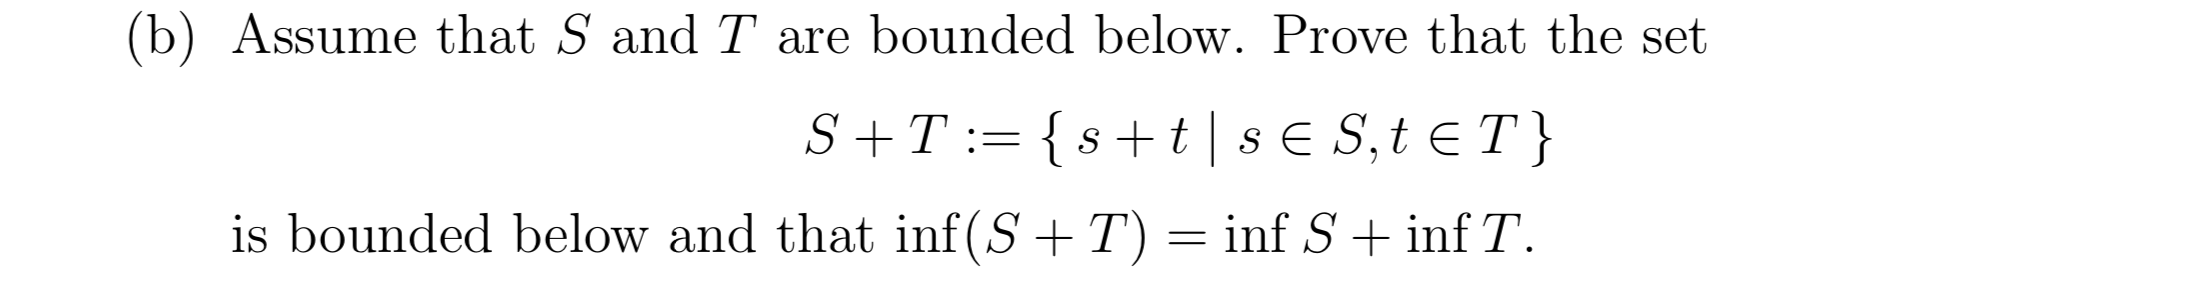
\includegraphics[width=400pt]{img/oxford-M2-analysis-I-2-5-b.png}
\end{mdframed}

\begin{proof}
  Let $S, T \subset \R$ with $S, T \neq \emptyset$. Assume that $S$ and $T$ are bounded
  below. Then $\inf S$ and $\inf T$ exist. Define
  \begin{align*}
    S + T := \{s + t ~|~ s \in S, t \in T\}.
  \end{align*}
  Let $a = \inf S + \inf T$.

  We claim that $a$ is a lower bound for $S + T$, i.e. $u \geq a$ for all $u \in S + T$.

  Let $u \in S + T$. Then $u = s + t$ for some $s \in S, t \in T$. Therefore
  $$u = (\inf S + v) + (\inf T + w) = a + (v + w) \geq a$$ for some $v, w \geq 0$. Therefore $a$ is
  a lower bound for $S + T$ as claimed.

  We further claim that $a = \inf S + T$.

  Suppose for a contradiction that there exists $b > a$ such that $b$ is a lower bound for
  $S + T$. Then $$b = a + v + w = (\inf S + v) + (\inf T + w)$$ for some $v, w > 0$. Fix
  $0 < \delta < \min(v, w)$. By {\bf 4.9} (Approximation Property of the supremum/infimum) there
  exist $s \in S$ and $t \in T$ such that $\inf S \leq s < \inf S + \delta$ and
  $\inf T \leq t < \inf T + \delta$. But then $s + t \in S + T$ and $s + t < b$, so $b$ is not a
  lower bound for $S + T$, a contradiction. Therefore $a = \inf S + T$ as claimed.
\end{proof}

\newpage
\subsection{}
\begin{mdframed}
  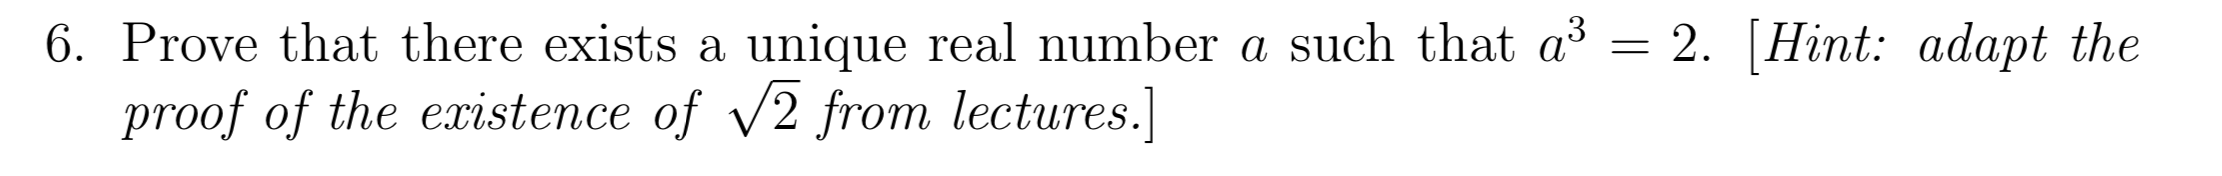
\includegraphics[width=400pt]{img/oxford-M2-analysis-I-2-6.png}
\end{mdframed}

\begin{proof}
  Let $S = \{x \in \R ~|~ x^3 < 2\}$. Since $S$ is bounded above, $\sup S$ exists. Let
  $a = \sup S$. By trichotomy it suffices to show that $a^3 < 2$ and $a^3 > 2$ lead to
  contradictions.

  First suppose $a^3 < 2$. We seek $h > 0$ such that $(a + h)^3 < 2$ since then $a + h \in S$,
  which would contradict the definition $a := \sup S$. Note that
  \begin{align*}
    (a + h)^3 &= a^3 + 3a^2h + 3ah^2 + h^3 - 2\\
              &< a^3 + 7a^2h - 2 ~~~~~~~~~~~~~~~~~~~~~~~~\text{if $h < a$}\\
              &< 0              ~~~~~~~~~~~~~~~~~~~~~~~~~~~~~~~~~~~~~~~~~\text{if $h < \frac{2 - a^3}{7a^2}$},
  \end{align*}
  therefore if we take $h < \min\(a, \frac{2 - a^3}{7a^2}\)$ then we have the desired
  contradiction.

  Alternatively suppose that $a^3 > 2$. By the Approximation Property for all $0 < h < a$ we can
  find $s \in S$ such that $a - h < s$, therefore $(a - h)^3 < s^3$. We seek an $h$ for which
  $(a - h)^3 > 2$ since then we would have $s^3 > 2$ which would contradict the definition of
  $S$. Note that
  \begin{align*}
    (a - h)^3 - 2 &= a^3 - 3a^2h + 3ah^2 - h^3 - 2\\
                  &> 0 ~~~~~~~~~~~~~~~~~~~~~~~~~~~~~~~~~~~~~~~~~\text{if $3ah^2 > 3a^2h + h^3$}.
  \end{align*}
  So we require $3ah > 3a^2 + h^2 \iff 3a^2 - 3ah + h^2 < 0$.

  \red{Incomplete}
\end{proof}

\newpage
\subsection{}
\begin{mdframed}
  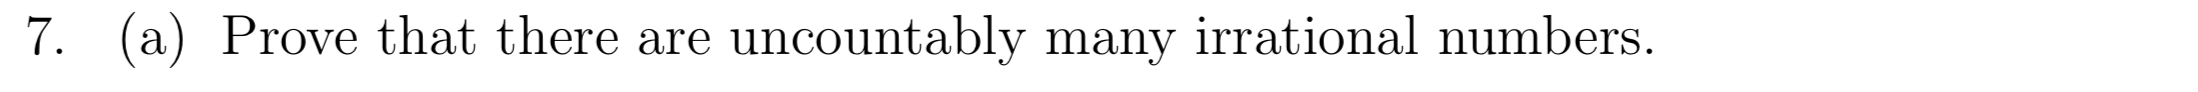
\includegraphics[width=400pt]{img/oxford-M2-analysis-I-2-7-a.png}
\end{mdframed}
\begin{definition*}[Countable]
  A set $S$ is countable if $S \preceq N$. I.e. there exists an injection $f:S \to \N$.
\end{definition*}
\begin{definition*}[Uncountable]
  A set $S$ is uncountable if it is not countable.
\end{definition*}
\begin{definition*}[Injection]
  A function $A \to B$ is an injection if $f(a_1) = f(a_2) \implies a_1 = a_2$.
\end{definition*}
\begin{proof}
  Suppose for a contradiction that $\R \setminus \Q$ is countable. Then an injection
  $f:\R \setminus \Q \to \N$ exists. Since $\Q$ is countable, an injection $g:\Q \to \N$
  exists. Consider the function $h:\R \to \N$ defined by
  \begin{align*}
    h(x) =
    \begin{cases}
      2f(x) &x \in \R \setminus \Q\\
      2g(x) + 1 &x \in \Q.
    \end{cases}
  \end{align*}
  We claim that $h:\R \to \N$ is an injection. Note that
  \begin{enumerate}[label=(\roman*)]
  \item $h(\R\setminus\Q) \cap h(\Q) = \emptyset$
  \item The $\R \to \R$ functions defined by $x \mapsto 2x$ and $x \mapsto 2x + 1$ are both
    injections.
  \item The composition of two injections is an injection.
  \end{enumerate}
  Suppose $h(x_1) = h(x_2)$. Then either $x_1, x_2 \in \Q$ or $x_1, x_2 \in \R\setminus\Q$ by
  (i). In both cases we have $x_1 = x_2$ by (ii) and (iii). Therefore $h:\R \to \N$ is an
  injection, hence $\R$ is countable.

  But $\R$ is not countable, so we have a contradiction. Therefore no such injection $f$ exists,
  i.e. $\R\setminus\Q$ is uncountable.
\end{proof}

\begin{lemma*}
  Let $a, b$ be real numbers with $a < b$. Let $\delta \in \R$ with $0 < \delta < b - a$. Then
  there exists $m \in \N$ such that $m\delta \in (a, b)$.
\end{lemma*}

\begin{proof}
  Let $m \in \N$, $\delta \in \R$ with $0 < \delta < b - a$, and define
  $S = \{m\delta ~|~ m\delta < b\}$. Note that $\delta \in S$. Therefore $S$ is non-empty, bounded
  above, and finite, hence $\max S$ exists.

  Let $M\delta = \max S$. We have $M\delta < b$. Suppose for a contradiction that $M\delta \leq
  a$. Recall that $\delta < b - a$. Summing these inequalities gives $(M + 1)\delta < b$. But then
  $M\delta \neq \max S$ since $(M + 1)\delta > M\delta$ and $(M + 1)\delta \in S$. This is a
  contradiction, therefore $M\delta \in (a, b)$.
\end{proof}

\begin{mdframed}
  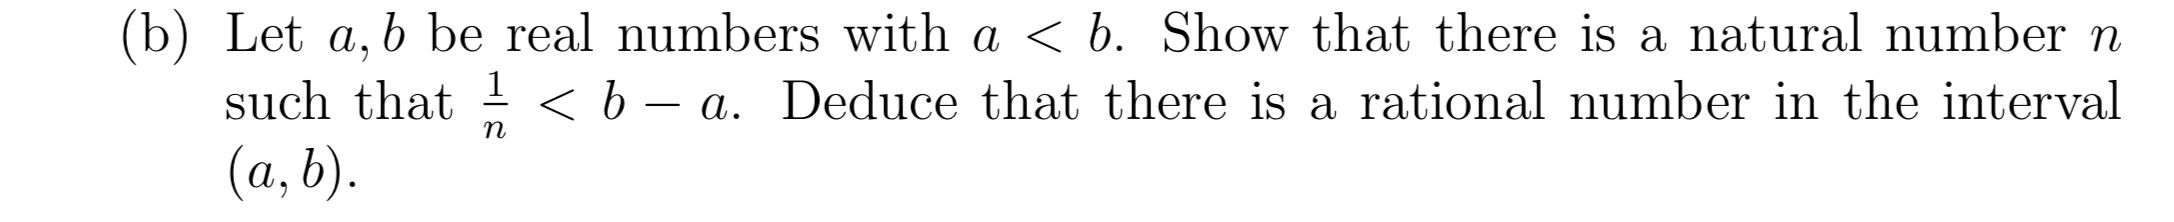
\includegraphics[width=400pt]{img/oxford-M2-analysis-I-2-7-b.png}
\end{mdframed}

\begin{proof}
  Let $a, b \in \R$ with $a < b$. Then $b - a > 0$. Since $\N$ is not bounded above (Archimedean
  property) there exists $n \in \N$ such that $n > 1/(b - a)$, therefore $1/n < b - a$. Therefore,
  by the lemma with $\delta = 1/n$, there exists $m \in \N$ such that $m/n \in (a, b) \cap \Q$.
\end{proof}

\begin{mdframed}
  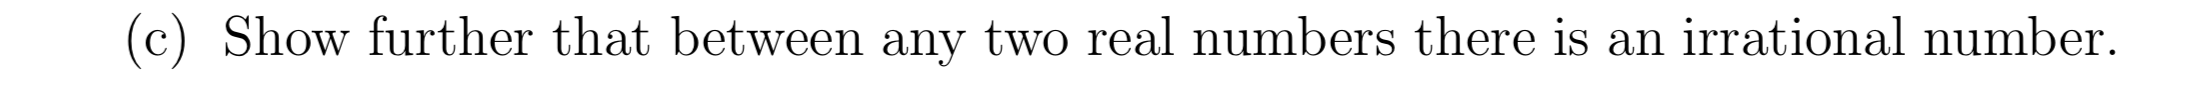
\includegraphics[width=400pt]{img/oxford-M2-analysis-I-2-7-c.png}
\end{mdframed}

\begin{proof}
  Let $a, b \in \R$ with $a < b$. By the Archimedean property of $\N$, there exists $n \in \N$ be
  such that $1/n < (b - a)/\pi$, therefore $\pi/n < (b - a)$. Therefore, by the lemma with
  $\delta = \pi/n$, there exists $m \in \N$ such that $m\pi/n \in (a, b) \cap (\R\setminus\Q)$.
\end{proof}
\newpage
\subsection{}
\begin{lemma*}
  The set of polynomials of degree $n$ with integer coefficients is countable.
\end{lemma*}
\begin{proof}
  Let $\{\alpha_1, \alpha_2, \ldots\}$ be the positive prime numbers and let
  $$P_n := \Big\{\sum_{i=0}^n a_iz^i ~|~ a_0, \ldots, a_n \in \Z, a_n \neq 0\Big\}$$ be the set of
  polynomials with integer coefficients of degree $n$. Note that
  $|P_n| = \big|\(\Z\setminus\{0\}\) \times \Z^{n-1}\big|$ and that
  $f:\(\Z\setminus\{0\}\) \times \Z^{n-1} \to \N$ given by
  \begin{align*}
    f(a_0, a_1, \ldots, a_n) = \prod_{i=0}^n\alpha_i^{a_i}\
  \end{align*}
  is a bijection by uniqueness of prime factorization of the natural numbers. Therefore $P_n$ is
  countable.
\end{proof}

\begin{mdframed}
  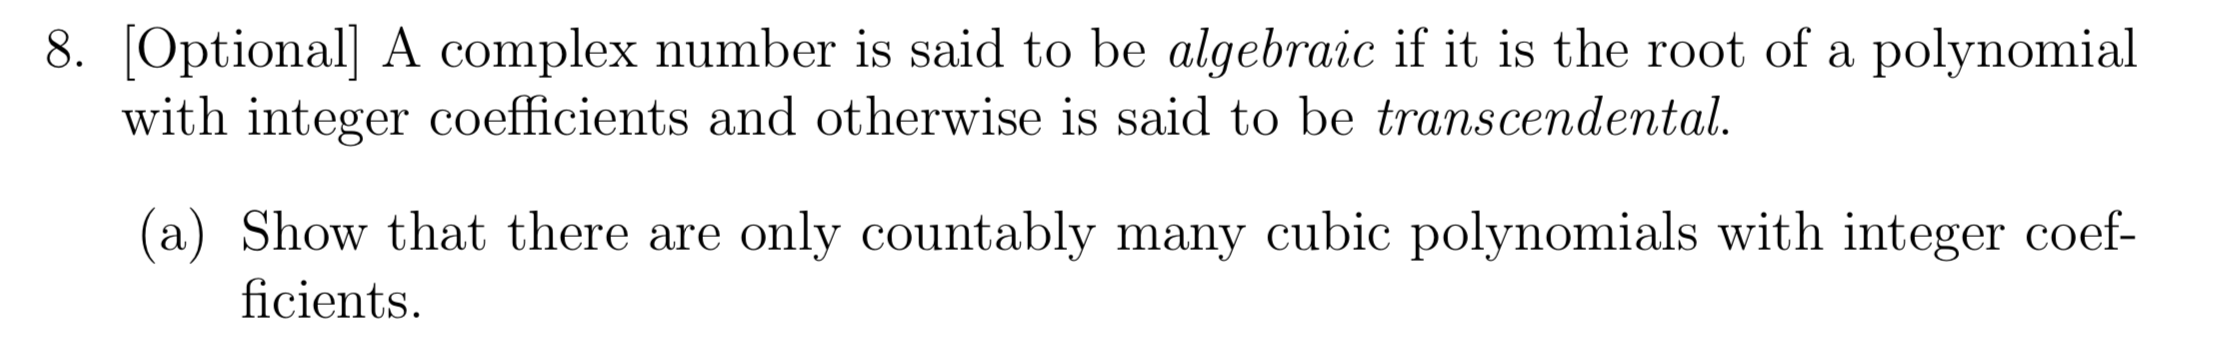
\includegraphics[width=400pt]{img/oxford-M2-analysis-I-2-8-a.png}
\end{mdframed}

\begin{proof}
  This follows from the lemma with $n=3$.
\end{proof}

\begin{lemma*}[Countable union of countable sets is countable]~\\
  Let $I \subseteq \N$ and let $S_i$ be a countable set for all $i \in I$. Then
  $\bigcup_{i\in I}S_i$ is countable.
\end{lemma*}
\begin{proof}
  Let $s_{ij}$ be the $j$-th element of $S_i$. The $f:\bigcup_{i\in I}S_i \to \N$ given by
  \begin{align*}
    f(s_{ij}) = 2^i3^j
  \end{align*}
  is a bijection, proving that $\bigcup_{i\in I}S_i$ is countable.
  \red{But what about repeated elements?}
\end{proof}

\begin{mdframed}
  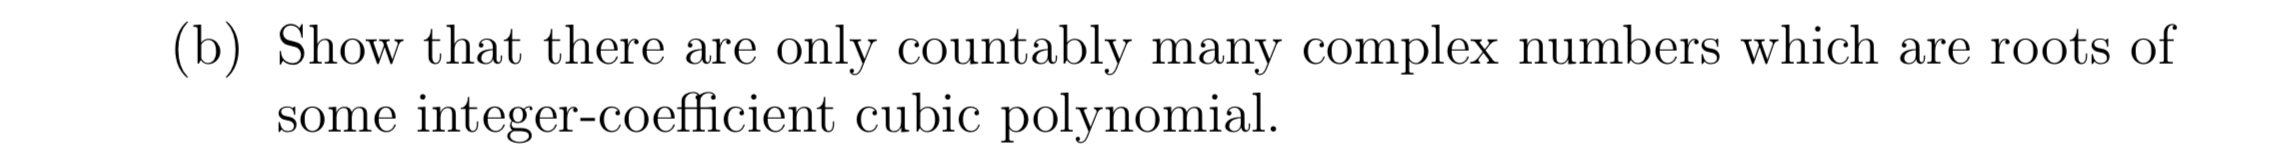
\includegraphics[width=400pt]{img/oxford-M2-analysis-I-2-8-b.png}
\end{mdframed}

\begin{lemma*}
  Let $P_n$ be the set of polynomials with integer coefficients of degree $n$. Then the set of
  complex numbers that are roots of a polynomial in $P_n$ is countable.
\end{lemma*}
\begin{proof}
  Let $P_{n,k}$ be the set of polynomials of degree $n$ that have $k \leq n$ distinct roots. Since
  $P_{n,k} \subseteq P_n$, we have that $P_{n,k}$ is countable. Therefore For each polynomial in
  $P_{n,k}$ order the $k$ distinct roots and label them $1, \ldots, k$. Then $P_{n,k}$ is countable
  since...
\end{proof}

\begin{proof}
  Note that a cubic polynomial has at most 3 distinct roots.

  Let $U$ be the set of complex numbers that are roots of some integer-coefficient cubic
  polynomial. For each such polynomial, assign a distinct label from $\{0, 1, 2\}$ to each of the
  distinct roots. Then the cardinality of $U$ is equal(*) to the cardinality of
  $B := \Z\setminus\{0\} \times \Z^3 \times \{0, 1, 2\}$. The set $B$ is countable since
  $f:T \to \N$ given by $f(a, b, c, d, e) = 2^a3^b5^c7^d11^e$ is an injection. (\red{* How to
    properly deal with the fact that $U$ is smaller than $B$ due to some polynomials having fewer
    than 3 distinct roots?})
\end{proof}

\begin{mdframed}
  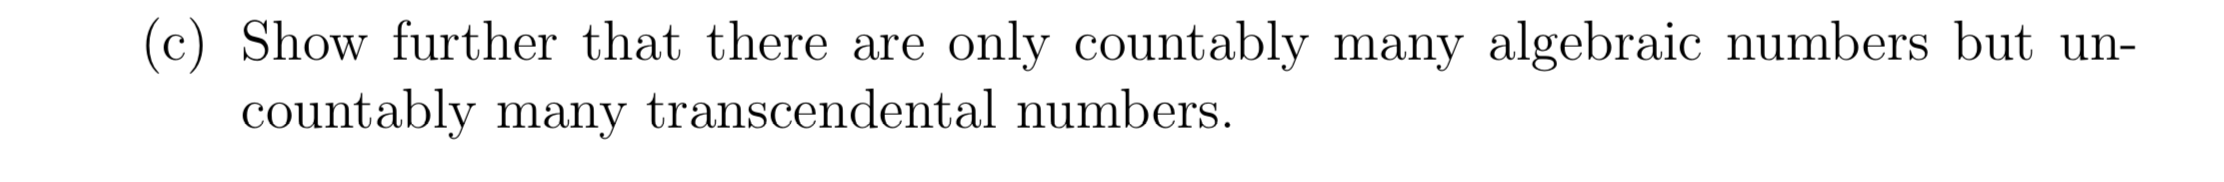
\includegraphics[width=400pt]{img/oxford-M2-analysis-I-2-8-c.png}
\end{mdframed}

\begin{proof}
  Let $A_n$ be the set of complex numbers which are roots of a polynomial of degree $n$.

  Claim: $A_n$ is countable for all $n \in \N$, since there are countably many polynomials of
  degree $n$ and each has a finite number of roots.

  The set of algebraic numbers is $A := \cup_{n\in\N} A_n$. Let $a_{ijk}$ be the $k$-th distinct
  root of the $j$-th polynomial of degree $i$. Then $f:$

  (This differs because whereas previously we were restricted to cubics, now the polynomials can
  be of any degree $n \in \N$.)

  The cardinality of the set of algebraic numbers is \red{Incomplete}.
\end{proof}
\newpage
\section{Sheet 3}

\subsection{}
\begin{mdframed}
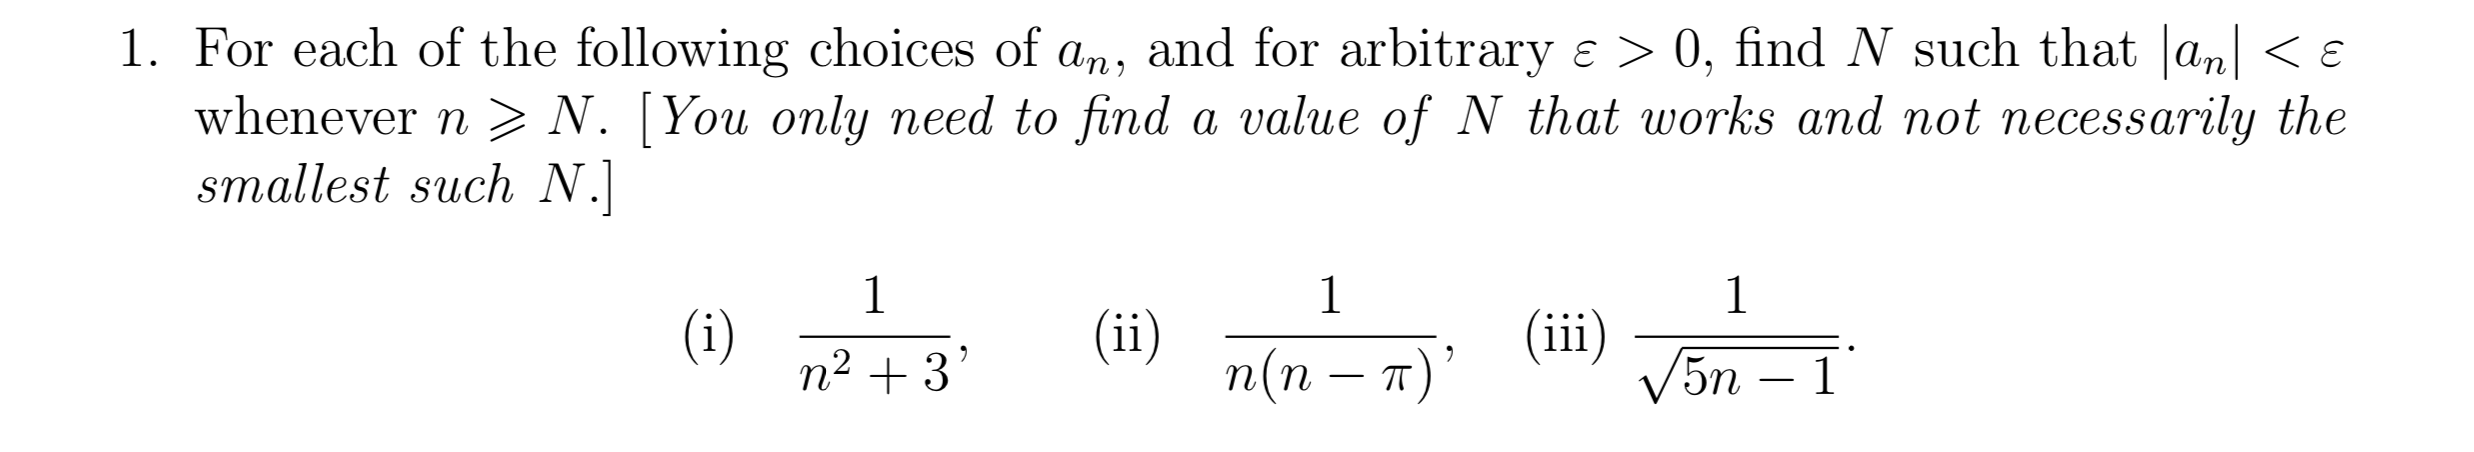
\includegraphics[width=400pt]{img/oxford-M2-analysis-I-3-1.png}
\end{mdframed}

\begin{enumerate}[label=(\roman*)]
\item Take $n = \ceil{\frac{1}{\sqrt{\epsilon}}}$. Then
  $
    |a_n| < \frac{1}{\ceil{\frac{1}{\sqrt{\epsilon}}}^2}
          \leq \frac{1}{\frac{1}{\epsilon}}
          = \epsilon.
  $
  Therefore $N = \ceil{\frac{1}{\sqrt{\epsilon}}}$ works.
\item Note that $|n(n - \pi)| = n|n - \pi| > n$ for $n \geq 4$. Therefore
  \begin{align*}
    |a_n| = \frac{1}{|n(n - \pi)|} &< \frac{1}{n} ~~~~~~~\text{if $n \geq 4$}\\
                                   &< \epsilon    ~~~~~~~\text{if $n > \Bigceil{\frac{1}{\epsilon}}$}.
  \end{align*}
  Therefore $N = \max\(1 + \Bigceil{\frac{1}{\epsilon}}, 4\)$ works.
\item Take $n = \Bigceil{\frac{1}{5\epsilon^2} + \frac{1}{5}}$. Then $|a_n| \leq
  \epsilon$. Therefore $N = \Bigceil{\frac{1}{5\epsilon^2}} + 1$ works.
\end{enumerate}

\newpage
\subsection{}
\begin{mdframed}
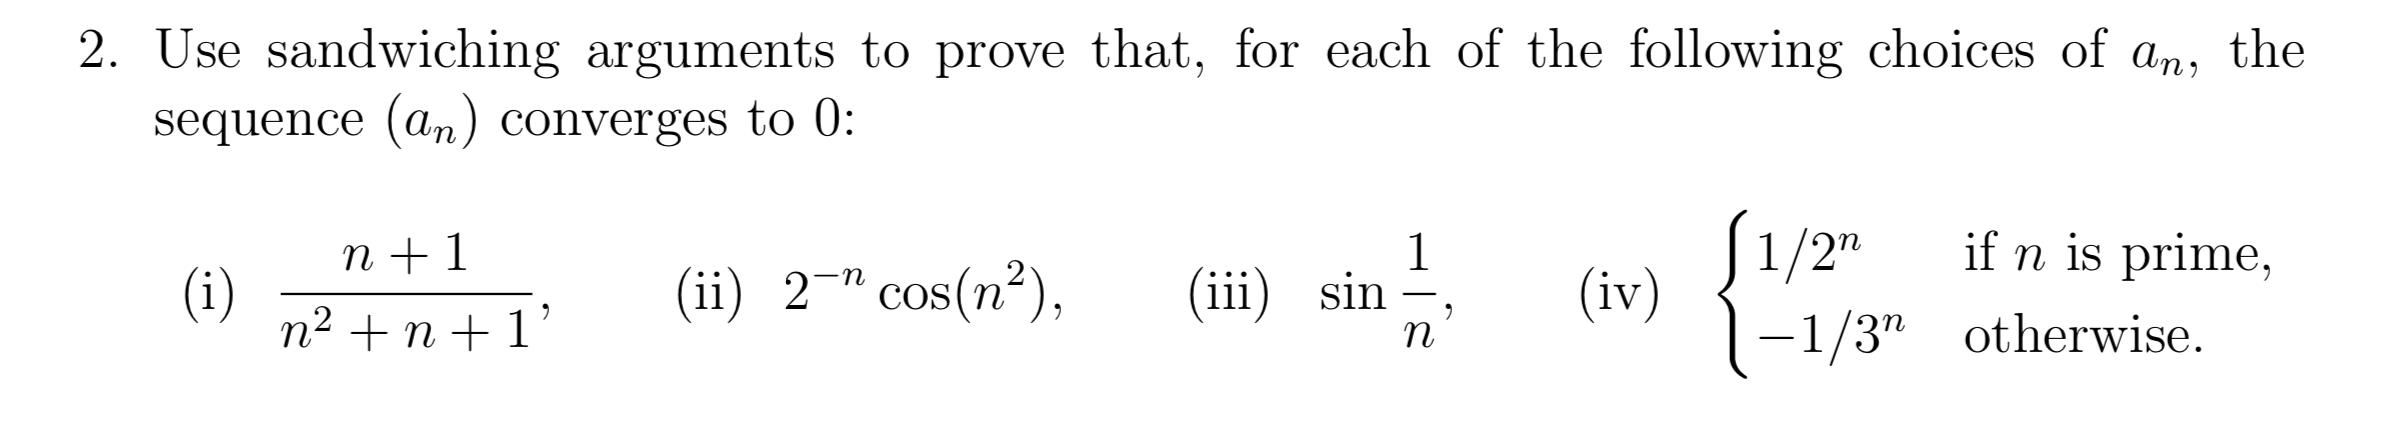
\includegraphics[width=400pt]{img/oxford-M2-analysis-I-3-2.png}
\end{mdframed}

\begin{enumerate}[label=(\roman*)]
\item Note that
  \begin{align*}
    0 < a_n
    = \frac{n + 1}{n^2 + n + 1}
    = \frac{1}{n + 1 + 1/n} + \frac{1}{n^2 + n + 1}
    < \frac{1}{n} + \frac{1}{n^2}.
  \end{align*}
  Therefore $a_n \to 0$, since $\frac{1}{n} + \frac{1}{n^2} \to 0$.
\item Note that $\cos n^2$ is bounded and that $2^{-n} \to 0$. Therefore
  $a_n = 2^{-n}\cos n^2 \to 0$.
\item Note that $0 \leq \sin x \leq x$ for all $0 \leq x \leq \pi$. Therefore
  $0 \leq a_n = \sin \frac{1}{n} \leq \frac{1}{n}$. We have $\frac{1}{n} \to 0$, therefore
  $a_n \to 0$ by the Sandwiching Lemma and the Tails Lemma.
\item Note that $-\frac{1}{3^n} \leq a_n \leq \frac{1}{2^n}$. Therefore by $a_n \to 0$ by the
  Sandwiching Lemma since $-\frac{1}{3^n} \to 0$ and $\frac{1}{2^n} \to 0$.
\end{enumerate}

\newpage
\subsection{}
\begin{mdframed}
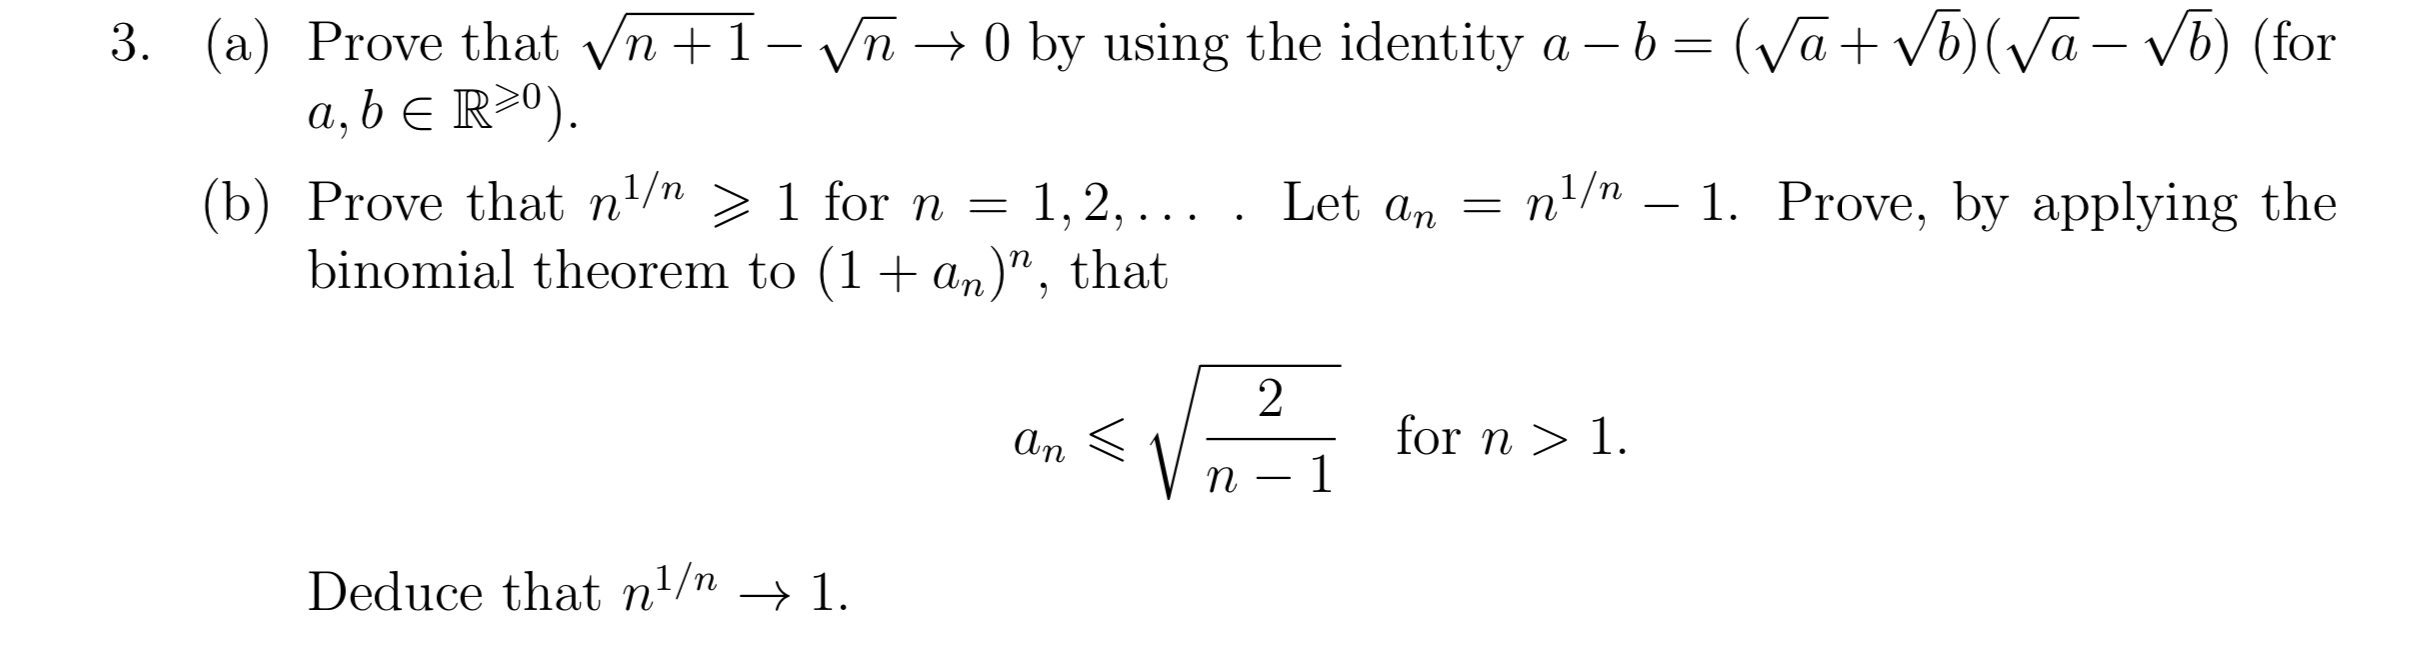
\includegraphics[width=400pt]{img/oxford-M2-analysis-I-3-3.png}
\end{mdframed}

\begin{enumerate}[label=(\alph*)]
\item
  \begin{claim*}
    $\sqrt{n+1} - \sqrt{n} \to 0$.
  \end{claim*}

  \begin{proof}
    Note that for $n \geq 1$
    \begin{align*}
      \sqrt{n+1} - \sqrt{n}
      = \frac{n + 1 - n}{\sqrt{n+1} + \sqrt{n}}
      = \frac{1}{\sqrt{n+1}} + \frac{1}{\sqrt{n}}.
    \end{align*}
    Further, note that $\frac{1}{\sqrt{n}} \to 0$ since for all $\epsilon > 0$ if
    $n \geq \ceil{\frac{1}{\epsilon^2}} + 1$ we have $\frac{1}{\sqrt{n}} < \epsilon$.

    Also $0 < \frac{1}{\sqrt{n+1}} < \frac{1}{\sqrt{n}}$ therefore $\frac{1}{\sqrt{n+1}} \to 0$ by
    the Sandwiching Lemma.

    Therefore $\sqrt{n+1} - \sqrt{n} \to 0 + 0 = 0$ by Algebra of Limits.
  \end{proof}
\item
  \begin{claim*}
    $n^{1/n} \geq 1$ for $n = 1, 2, \ldots$.
  \end{claim*}
  \begin{proof}
    Suppose there exists $n \in \N$ such that $n^{1/n} < 1$. Let $\alpha = n^{1/n} < 1$. Then
    $\alpha^n \geq 1$ since $\(n^{1/n}\)^n = n \in \N$. But we can prove by induction that
    $\alpha^n < 1$: We have $\alpha^1 < 1$; suppose $\alpha^k < 1$. Then
    $\alpha^{k+1} = \alpha\alpha^k < 1$. Therefore $\alpha^n < 1$ for $n = 1, 2, \ldots$ by
    induction. This contradiction proves that $n^{1/n} \geq 1$ for $n = 1, 2, \ldots$.
  \end{proof}

  \begin{claim*}
    Let $a_n = n^{1/n} - 1$. Then $a_n \leq \sqrt{\frac{2}{n - 1}}$ for $n > 1$.
  \end{claim*}
  \begin{proof}
    Note that $n = (1 + a_n)^n \geq 1 + na_n + \frac{n(n-1)}{2}a_n^2$. Therefore for $n > 1$ we
    have $\frac{n(n-1)}{2}a_n^2 \leq n$, therefore $a_n \leq \sqrt{\frac{2}{n - 1}}$.
  \end{proof}
  \begin{claim*}
    $n^{1/n} \to 1$.
  \end{claim*}
  \begin{proof}
    Fix $\epsilon > 0$. Note that if $n = \ceil{\frac{1}{2\epsilon^2}} + 1$ then
    $0 < \sqrt{\frac{2}{n - 1}} \leq \epsilon$. Let $N = \ceil{\frac{1}{2\epsilon^2}} + 2$. Then
    $|a_n - 0| < \epsilon$ for all $n \geq N$. Therefore $a_n \to 0$ and $n^\frac{1}{n} \to 1$.
  \end{proof}
\end{enumerate}


\newpage
\subsection{}
\begin{enumerate}[label=(\alph*)]
\item\hspace{0pt}
  \begin{mdframed}
    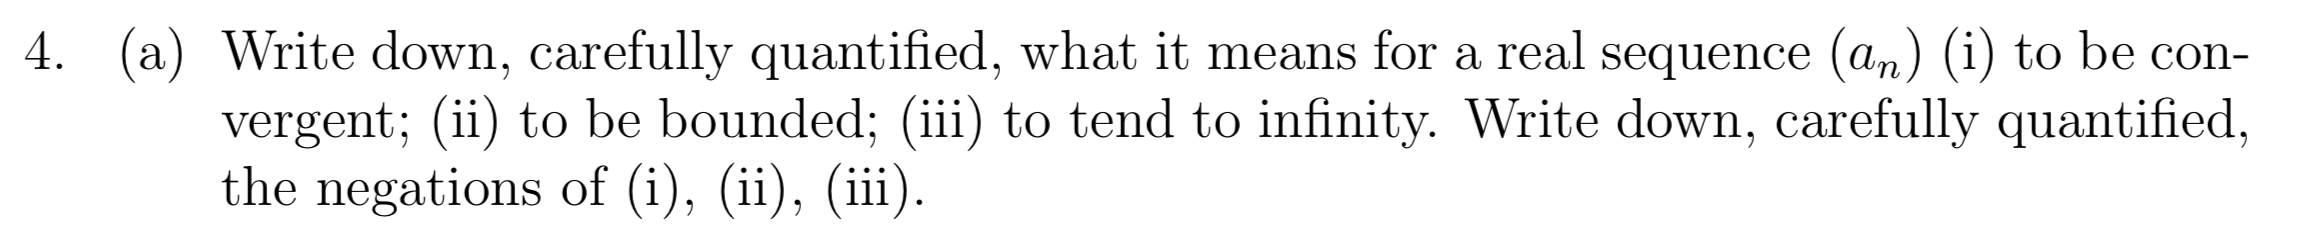
\includegraphics[width=400pt]{img/oxford-M2-analysis-I-3-4-a.png}
  \end{mdframed}
  \begin{definition*}\hspace{0pt}
    \begin{enumerate}[label=(\roman*)]
    \item $(a_n)$ is convergent if there exists $L \in \R$ such that for all $\epsilon > 0$ there
      exists $N \in \N$ such that $|a_n - L| < \epsilon$ for all $n \geq N$:
      \begin{align*}
        \exists L \in \R ~~ \forall \epsilon > 0 ~~ \exists N \in \N ~~ \forall n \geq N ~~ |a_n - L| < \epsilon.
      \end{align*}
      $(a_n)$ is not convergent if for all $L \in \R$ there exists $\epsilon > 0$ such that ``no
      $N$ works'':
      \begin{align*}
        \forall L \in \R ~~ \exists \epsilon > 0 ~~ \forall N \in \N ~~ \exists n \geq N ~~ |a_n - L| \geq \epsilon.
      \end{align*}
    \item $(a_n)$ is bounded if there exists $M \in \R$ such that $|a_n| < M$ for all $n \in \N$:
      \begin{align*}
        \exists M \in \R ~~ \forall n \in \N ~~ |a_n| < M.
      \end{align*}
      $(a_n)$ is not bounded if no $M \in \R$ is a bound:
      \begin{align*}
        \forall M \in \R ~~ \exists n \in \N ~~ |a_n| \geq M.
      \end{align*}
    \item $(a_n)$ tends to infinity if for all $M \in \R$ there exists $N \in \N$ such that $a_n > M$ for
      all $n \geq N$:
      \begin{align*}
        \forall M \in \R ~~ \exists N \in \N ~~ \forall n \geq N ~~ a_n > M.
      \end{align*}
      $(a_n)$ does not tend to infinity if there exists $M \in \R$ such that ``no $N$ works'':
      \begin{align*}
        \exists M \in \R ~~ \forall N \in \N ~~ \exists n \geq N ~~ a_n \leq M.
      \end{align*}
    \end{enumerate}
  \end{definition*}
\item\hspace{0pt}
  \begin{mdframed}
    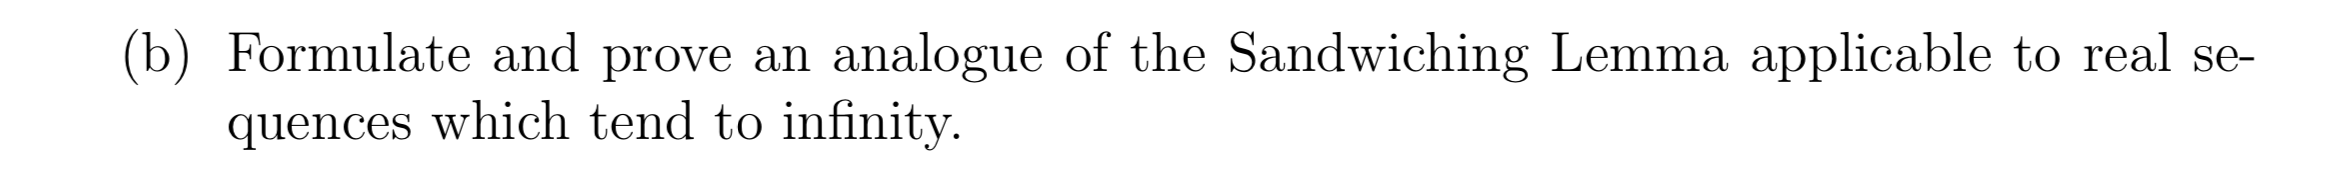
\includegraphics[width=400pt]{img/oxford-M2-analysis-I-3-4-b.png}
  \end{mdframed}
  \begin{claim*}
    Let $(a_n) \in \R^\N$ and let $(b_n) \in \R^\N$ tend to infinity. If $a_n \geq b_n$ for all
    $n \in \N$ then $a_n$ tends to infinity.
  \end{claim*}
  \begin{proof}
    Let $(a_n) \in \R^\N$ and let $(b_n) \in \R^\N$ tend to infinity. Suppose $a_n \geq b_n$ for
    all $n \in \N$.

    Let $M \in \R$.

    For $(b_n)$ we know there is an $N$ that works for $M$.

    Let $N$ be such that it works for $(b_n)$.

    Then $a_n \geq b_n > M$ for all $n \geq N$.
  \end{proof}
\newpage
\item\hspace{0pt}
  \begin{mdframed}
    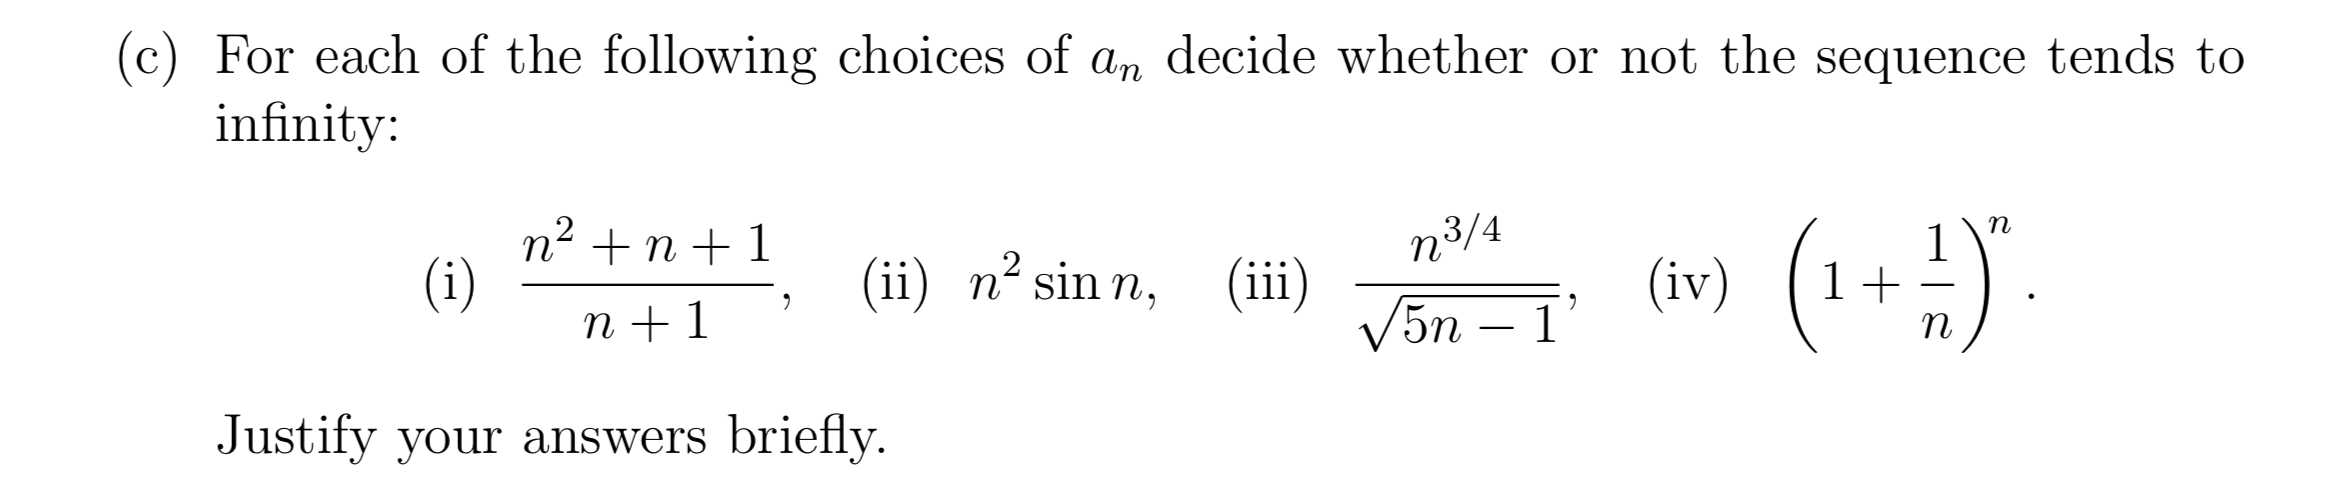
\includegraphics[width=400pt]{img/oxford-M2-analysis-I-3-4-c.png}
  \end{mdframed}
  \begin{definition*}~\\
    $(a_n)$ tends to infinity if
    \begin{align*}
      (\forall M \in \R) ~~ (\exists N \in \N) ~~ (\forall n \geq N) ~~ (a_n > M)
    \end{align*}
    $(a_n)$ does not tend to infinity if
    \begin{align*}
      (\exists M \in \R) ~~ (\forall N \in \N) ~~ (\exists n \geq N) ~~ (a_n \leq M)
    \end{align*}
  \end{definition*}
  \begin{enumerate}[label=(\roman*)]
  \item $a_n = \frac{n^2 + n + 1}{n + 1} > \frac{n^2}{n + 1} = \frac{n}{1 + 1/n}$.

    trick:
    $\frac{n^2}{n + 1} \geq \frac{n^2}{n + n}$


    Let $b_n = \frac{n}{1 + 1/n}$. Then $\frac{1}{b_n} = \frac{1}{n} + \frac{1}{n^2} \to
    0$.

    Therefore (theorem) $b_n \to \infty$, therefore $a_n \to \infty$.
    \red{Is there a better way to show this?}

  \item $a_n = n^2\sin n$.

    This does not tend to infinity since $\{n ~|~ n^2\sin n < 0\}$ has no upper bound.
  \item $a_n = \frac{n^{3/4}}{\sqrt{5n - 1}} > \frac{n^{3/4}}{\sqrt{9n}} = \frac{1}{3}n^{1/4}$.

    This tends to infinity. Proof: Fix $M \in \R$ and Put $N = \ceil{(3M)^4} + 1$. Then
    $\frac{1}{3}n^{1/4} > M$ for all $n \geq N$.

  \item $a_n = (1 + \frac{1}{n})^n = 1 + n\frac{1}{n} + {n \choose 2}\frac{1}{n^2} + \ldots > 2$

    Prove by induction that less than 3?

    (This is equal to $e$ so, as a matter of fact, it doesn't tend to infinity.)

  \end{enumerate}
\end{enumerate}

\newpage
\subsection{}
\begin{mdframed}
  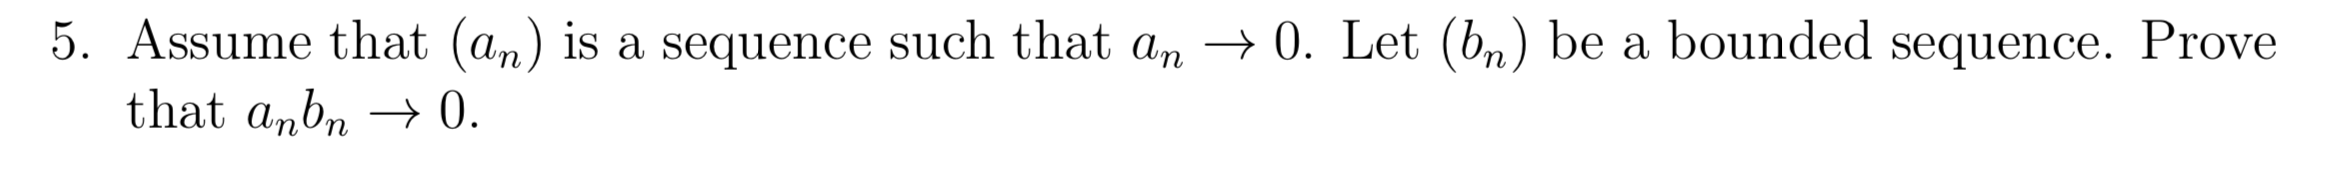
\includegraphics[width=400pt]{img/oxford-M2-analysis-I-3-5-1.png}
\end{mdframed}
\begin{claim*}
  Let $(a^n)$ be a sequence such that $a_n \to 0$. Let $(b_n)$ be a bounded sequence. Then
  $a_nb_n \to 0$.

  % I.e. $(\forall \epsilon > 0) ~~ (\exists N \in \N) ~~ (\forall n \geq N) ~~ (|a_nb_n| < \epsilon)$
\end{claim*}
\begin{proof}
  Let $(a^n)$ be a sequence such that $a_n \to 0$. Let $(b_n)$ be a bounded sequence.

  Let $M$ be a bound for $(b_n)$ so that $|b_n| \leq M$ for all $n$.

  Fix $\epsilon > 0$ and let $N$ be such that $|a_n| < \frac{\epsilon}{M}$ for all $n \geq N$.

  Then $|a_nb_n| = |a_n||b_n| < \epsilon$ for all $n \geq N$.
\end{proof}

\begin{mdframed}
  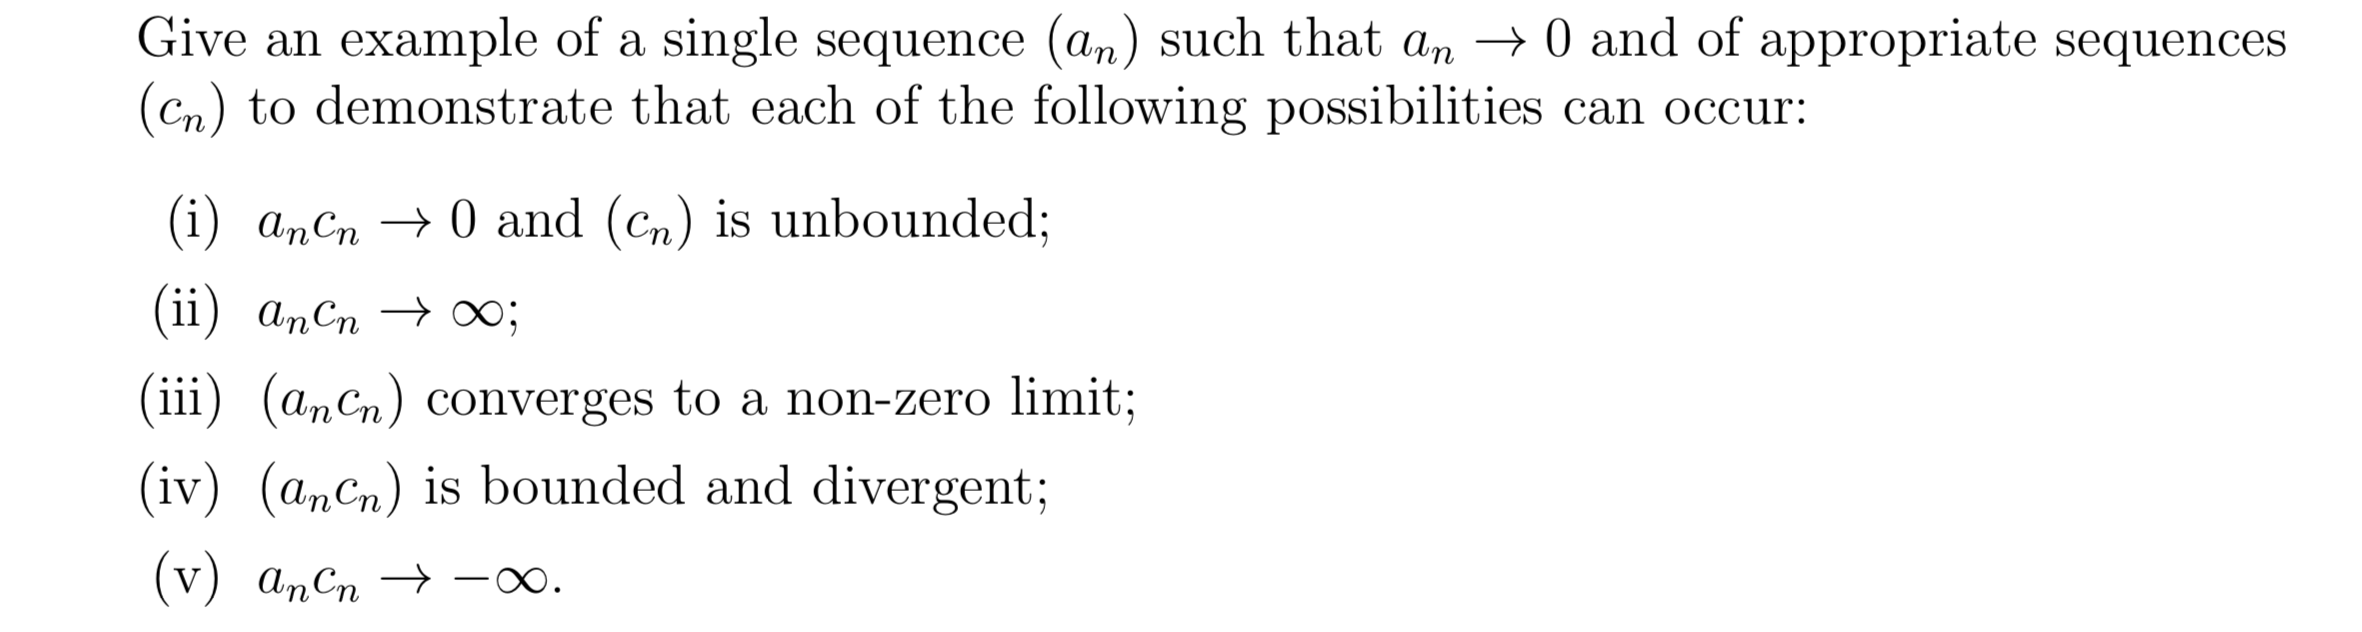
\includegraphics[width=400pt]{img/oxford-M2-analysis-I-3-5-2.png}
\end{mdframed}

\begin{enumerate}[label=(\roman*)]
\item Let $(c_n)$ be unbounded and let $a_n = 0$ for all $n$. Then $a_nc_n \to 0$.
\item Let $c_n = \frac{n}{a_n}$. Then $a_nc_n = n \to \infty$.
\item Let $L \neq 0$ and $c_n = \frac{L}{a_n}$. Then $a_nc_n = L$.
\item Let $c_n = \frac{\sin n}{a_n}$. Then $(a_nc_n) = (\sin n)$ which is bounded and divergent.
\item Let $c_n = \frac{-n}{a_n}$. Then $a_nc_n = n \to -\infty$.
\end{enumerate}

\newpage
\subsection{}
\begin{mdframed}
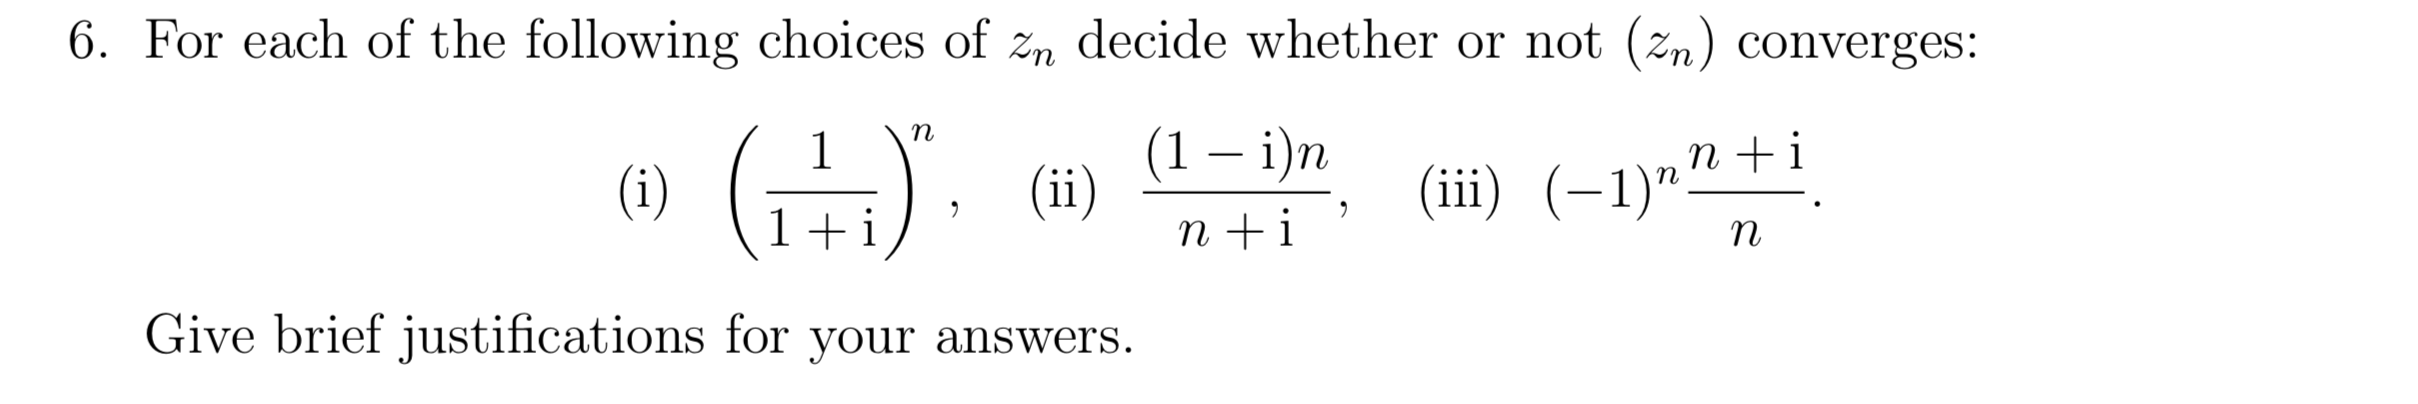
\includegraphics[width=400pt]{img/oxford-M2-analysis-I-3-6.png}
\end{mdframed}

\begin{enumerate}[label=(\roman*)]
\item
\end{enumerate}

\newpage
\subsection{}
\begin{mdframed}
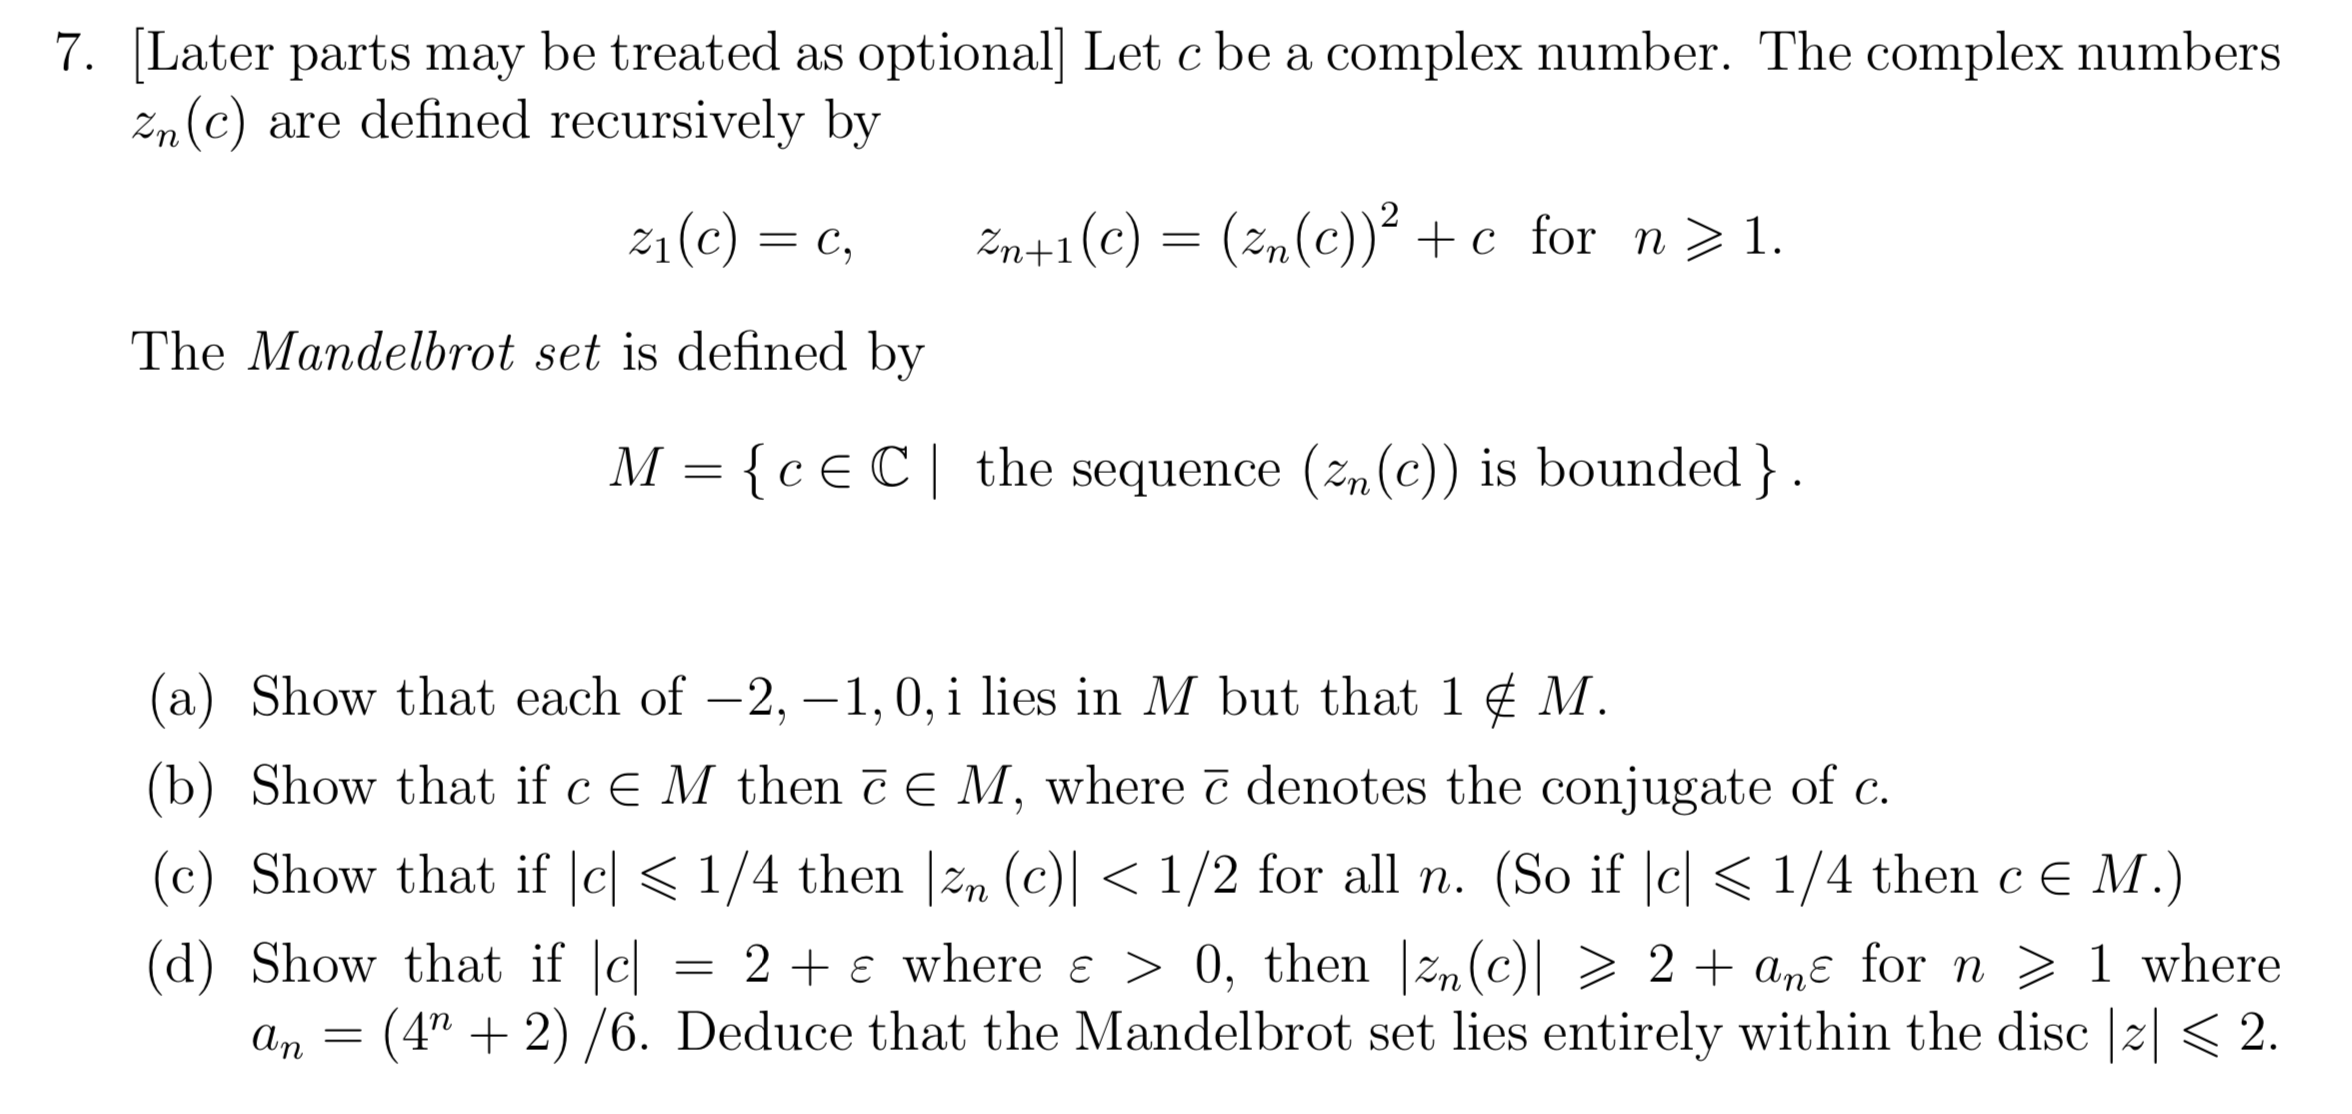
\includegraphics[width=400pt]{img/oxford-M2-analysis-I-3-7.png}
\end{mdframed}
\begin{enumerate}[label=(\alph*)]
\item
  $(z_n(-2)) = -2, 2, 2 \ldots$.\\
  Bounded (fixed point) therefore $-2 \in M$.

  $(z_n(-1)) = -1, 0, -1, \ldots$.\\
  Bounded (repeats) therefore $-1 \in M$.

  $(z_n(0)) = 0, -1, 0, \ldots$\\
  Bounded (repeats) therefore $-1 \in M$.

  $(z_n(i)) = i, -1 + i, -i, -1 + i, \ldots$\\
  Bounded (repeats) therefore $i \in M$.

  $(z_n(1)) = 1, 2, 5, 26, \ldots$\\
  Unbounded:\\
  Suppose for a contradiction that there exists $B$ such that
  $(\forall n \in \N) ~~ (|z_n(1)| \leq B)$. \red{incomplete}

\item
  Let $c \in M$. Let $B \in \C$ be such that $(\forall n \in \N) ~~ |z_n(c)| \leq B$.

  Note that $(\bar c)^2 = \bar{c^2}$. Therefore
  \[
    (z_n(c)) = c, c^2 + c,
    (z_n(\bar c)) = \bar c, \bar{c^2} + \bar{c}
  \]
\end{enumerate}


\newpage
\section{Sheet 4}
\subsection{}
\begin{enumerate}[label=(\alph*)]
\item~\\
  \begin{mdframed}
    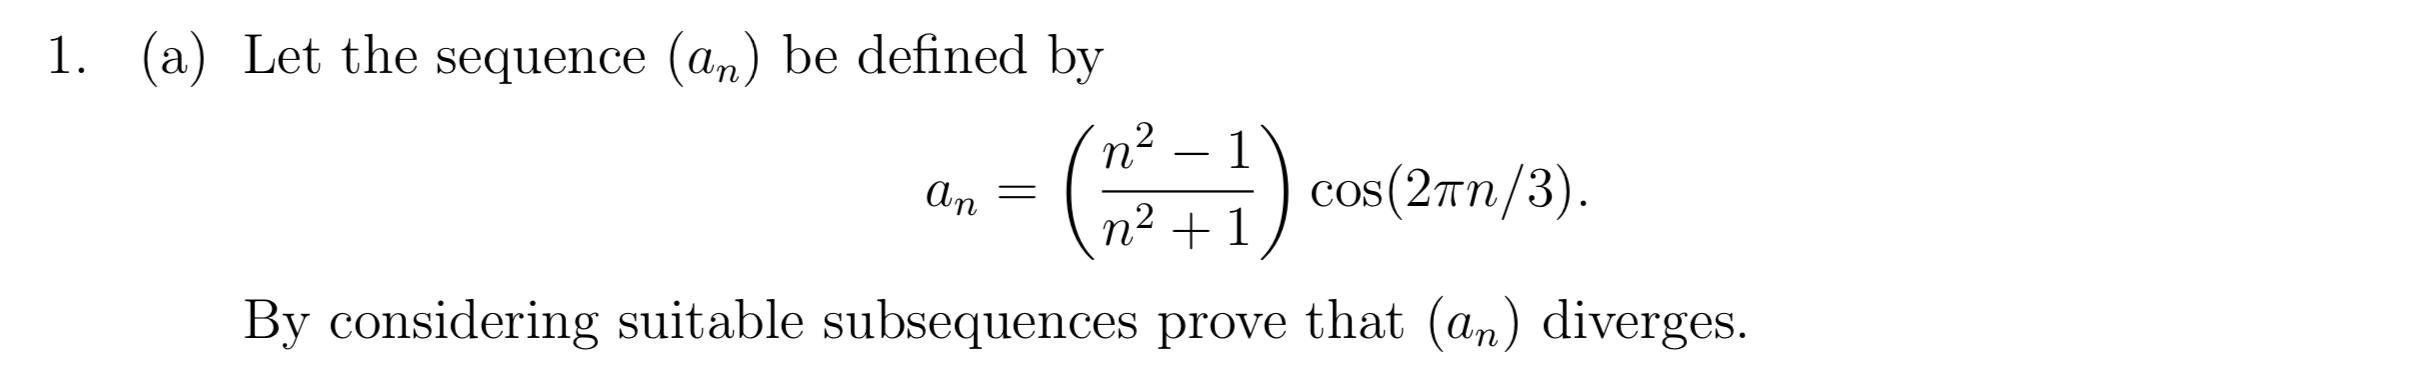
\includegraphics[width=400pt]{img/oxford-M2-analysis-I-4-1-a.png}
  \end{mdframed}

  Note that:
  \begin{enumerate}[label=(\arabic*)]
  \item $\frac{n^2 - 1}{n^2 + 1} = \frac{1 - n^{-2}}{1 + n^{-2}} \to 1$
  \item $\cos(\frac{2\pi n}{3})$ repeats with a period of 3. Therefore it diverges.
  \end{enumerate}

  Therefore $(a_n)$ diverges, since we can identify two constant subsequences within it with
  different constant values. I.e. they converge to different limits.
  \newpage
\item~\\
  \begin{mdframed}
    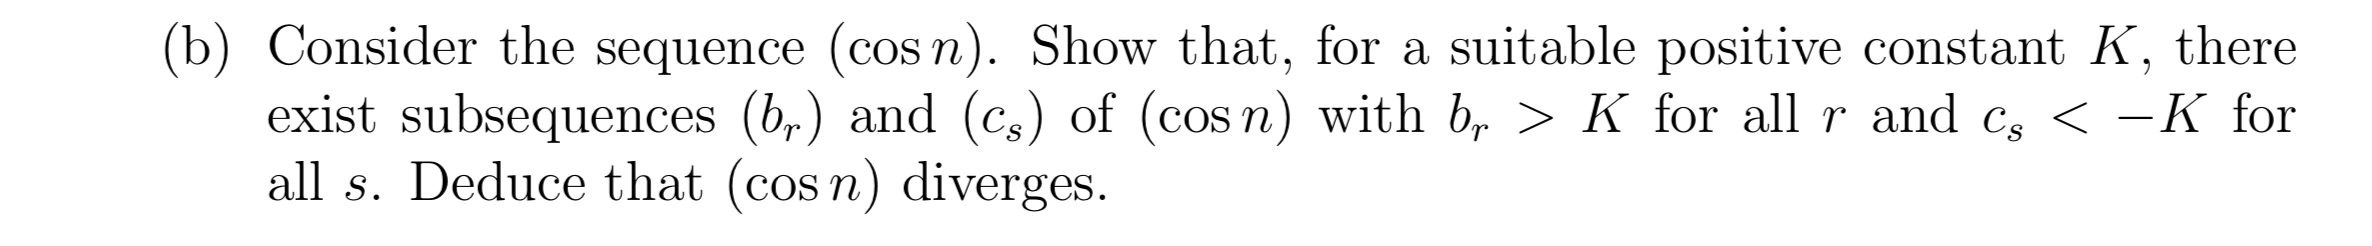
\includegraphics[width=400pt]{img/oxford-M2-analysis-I-4-1-b.png}
  \end{mdframed}

  \begin{proof}
    Let $K = \sqrt{\frac{1}{2}}$, let $n \in \N$ and let $x \in \R^{>0}$.

    Note that $|x - 2n\pi| < \frac{\pi}{4} \implies \cos(x) > K$. Let $f(n)$ be the smallest integer
    in $\(2n\pi - \frac{\pi}{4}, 2n\pi + \frac{\pi}{4}\)$ (the interval exceeds 1 in width therefore
    it contains at least one integer). Define $b_r = a_{f(r)}$. Then $b_r > K$ for all $r \in \N$.

    Similarly, note that $|x - (2n + 1)\pi| < \frac{\pi}{4} \implies \cos(x) < -K$. Let $g(n)$ be the
    smallest integer in $\((2n + 1)\pi - \frac{\pi}{4}, (2n + 1)\pi + \frac{\pi}{4}\)$ (the interval
    exceeds 1 in width therefore it contains at least one integer). Define $c_s = a_{g(s)}$. Then
    $c_s < -K$ for all $r \in \N$.

    Define
    \begin{align*}
      d_n =
      \begin{cases}
        b_n ~~~~\text{n odd}\\
        c_n ~~~~\text{n even}.
      \end{cases}
    \end{align*}
    Then $(d_n)$ does not converge since it is not Cauchy. But $(d_n)$ is a subsequence of $(a_n)$
    therefore $(a_n)$ does not converge.
  \end{proof}
\end{enumerate}


\newpage
\subsection{}
\begin{mdframed}
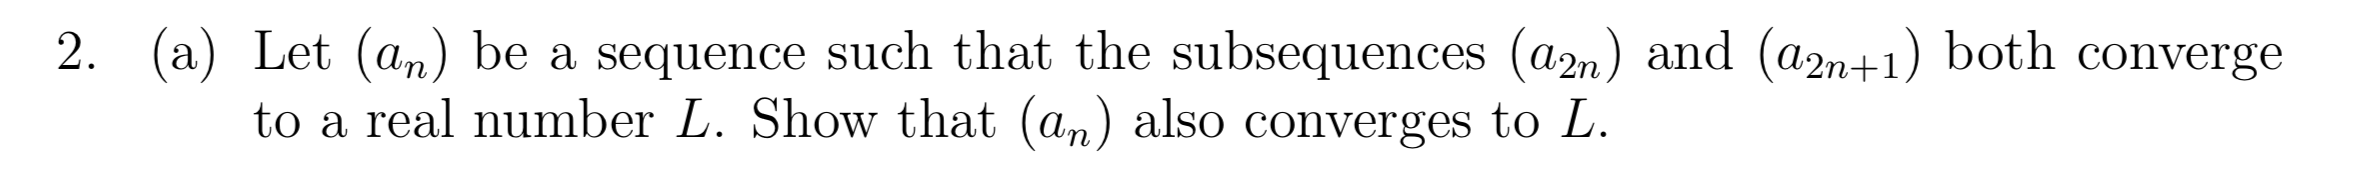
\includegraphics[width=400pt]{img/oxford-M2-analysis-I-4-2-a.png}
\end{mdframed}

\begin{proof}
  Let $(a_n)$ be such that $(a_{2n})$ and $(a_{2n + 1})$ both converge to $L \in \R$.

  Fix $\epsilon > 0$. Let $N_1 \in \N$ be such that $|a_{2n} - L| < \epsilon$ for all $n \geq N_1$
  and let $N_2 \in \N$ be such that $|a_{2n + 1} - L| < \epsilon$ for all $n \geq N_2$.

  Let $N = 2\max(N_1, N_2)$. Then $|a_n - L| < \epsilon$ for all $n \geq N$, therefore $a_n \to L$.
\end{proof}

\begin{mdframed}
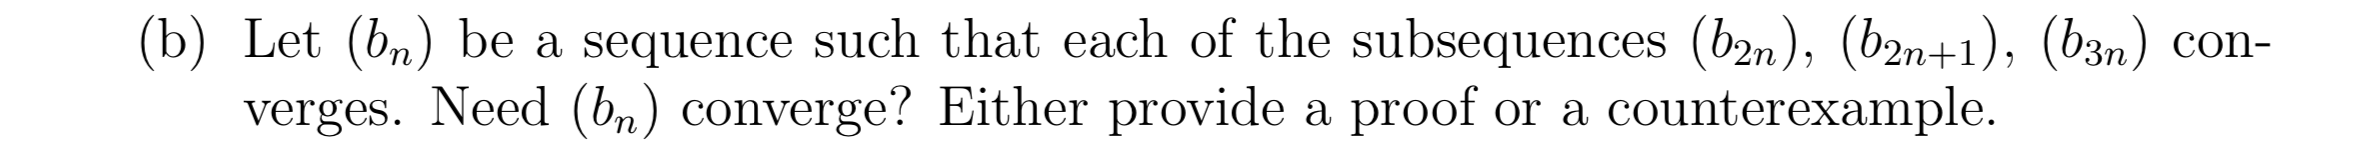
\includegraphics[width=400pt]{img/oxford-M2-analysis-I-4-2-b.png}
\end{mdframed}

Let $(b_{3n})$ converge to $L$. Therefore $(b_{6n})$ and $(b_{6n + 3})$ converge to $L$. Note that
$(b_{6n})$ is a subsequence of $(b_{2n})$, and $(b_{6n + 3})$ is a subsequence of $(b_{2n +
  1})$. It is given that $(b_{2n})$ and $(b_{2n + 1})$ converge, therefore they converge to $L$
also.

Therefore $(b_n)$ converges to $L$ by the result in part (a).

\begin{mdframed}
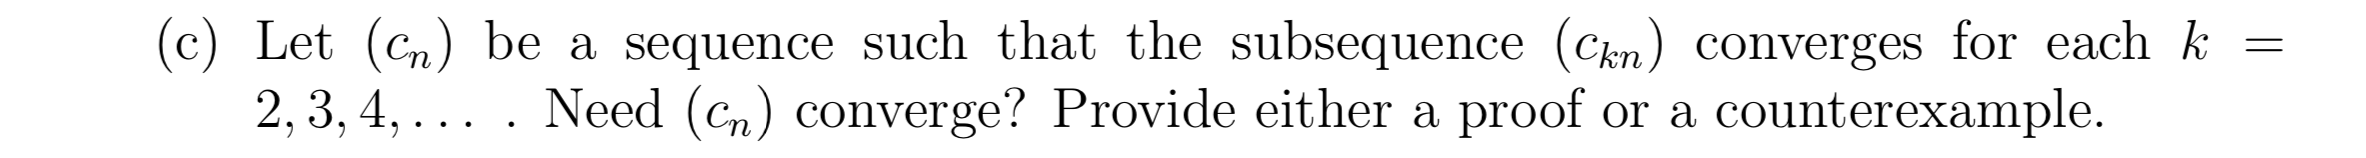
\includegraphics[width=400pt]{img/oxford-M2-analysis-I-4-2-c.png}
\end{mdframed}

\begin{proof}
  $c_n$ need not converge. As a counterexample define
  \begin{align*}
    c_n =
    \begin{cases}
      0 ~~~~~~~\text{$n$ prime}\\
      1 ~~~~~~~\text{otherwise}.
    \end{cases}
  \end{align*}
  This satisfies the description given of $(c_n)$ but is not Cauchy since the set of primes has no
  upper bound and the primes are interspersed with non-primes.
\end{proof}

\newpage
\subsection{}
\begin{mdframed}
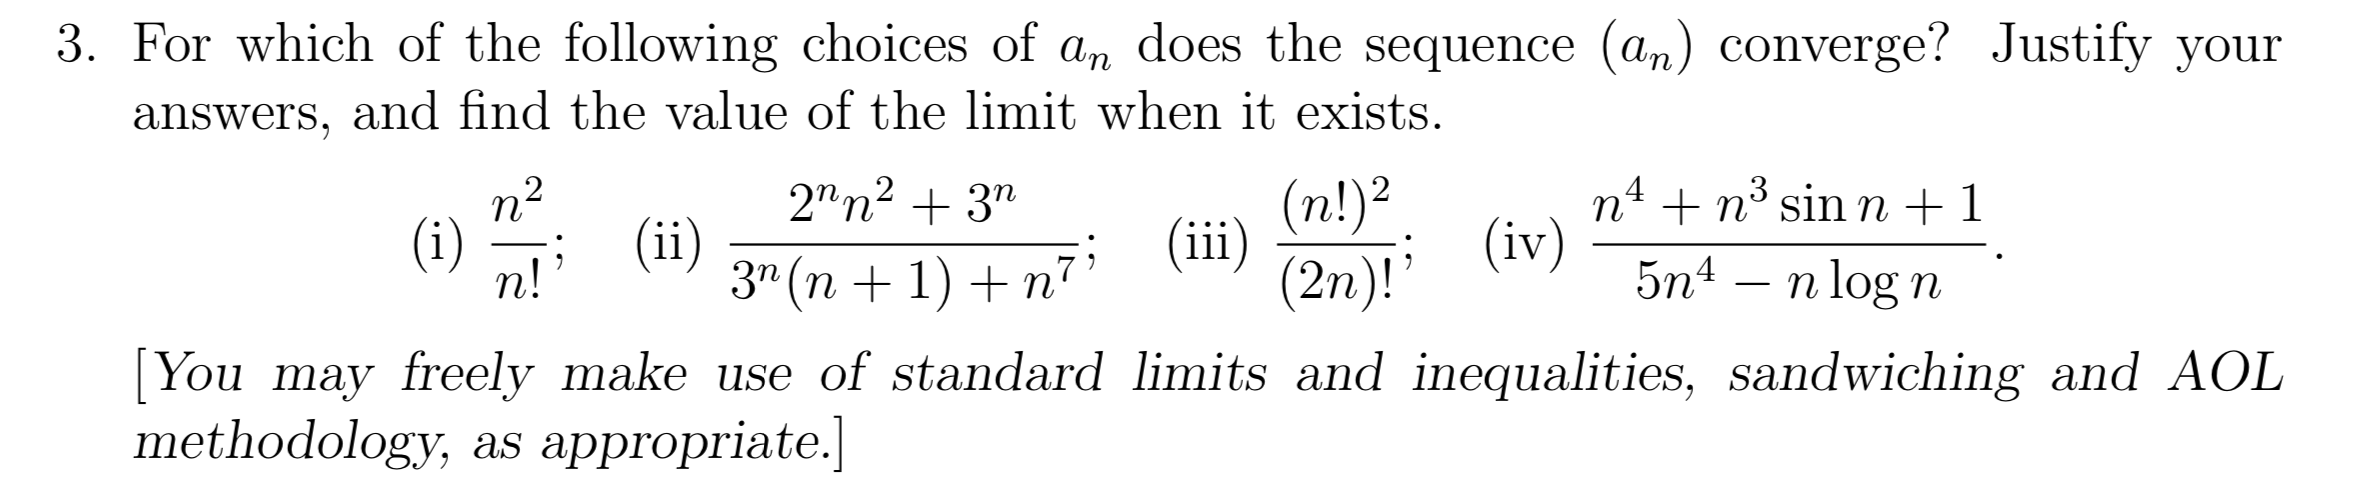
\includegraphics[width=400pt]{img/oxford-M2-analysis-I-4-3.png}
\end{mdframed}

\begin{enumerate}[label=(\roman*)]
\item
  \begin{align*}
    \frac{n^2}{n!} = \frac{n^2}{n(n-1)}\frac{1}{(n - 2)!} \to 1\cdot 0 = 0
  \end{align*}
% \item
%   \begin{align*}
%     \frac{2^nn^2 + 3^n}{3^n(n + 1) + n^7}
%   \end{align*}
\end{enumerate}


\newpage
\subsection{}
\begin{mdframed}
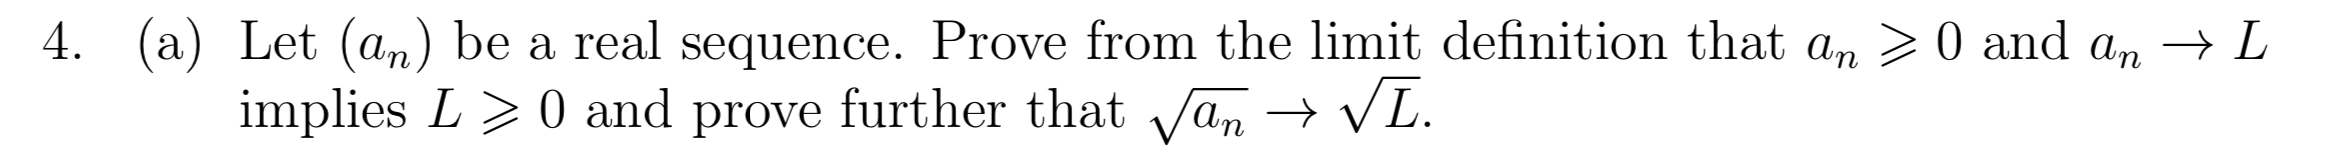
\includegraphics[width=400pt]{img/oxford-M2-analysis-I-4-4-a.png}
\end{mdframed}
\begin{enumerate}[label=(\alph*)]
\item Let $a_n \geq 0$ and $a_n \to L$.
  \begin{claim*}
    $L \geq 0$.
  \end{claim*}
  \begin{proof}
    Suppose for a contradiction that $L < 0$. Put $\epsilon = -\frac{L}{2} > 0$. Then there exists
    $N \in \N$ such that $|a_n - L| < \epsilon$ for all $n \geq N$. Let $n \geq N$. Then
    $a_n < L + \epsilon = L - \frac{L}{2} = \frac{L}{2} < 0$. But $a_n \geq 0$, a
    contradiction. Therefore $L \geq 0$.
  \end{proof}

  \begin{claim*}
    $\sqrt{a_n} \to \sqrt{L}$.
  \end{claim*}
  \begin{proof}
    It suffices to prove that $\sqrt{a_n} - \sqrt{L} \to 0$ since this is equivalent to
    $\sqrt{a_n} \to \sqrt{L}$.

    Note that $\sqrt{a_n} - \sqrt{L} = \frac{a_n - L}{\sqrt{a_n} + \sqrt{L}}$. By hypothesis, $a_n - L \to 0$.
\end{proof}

\end{enumerate}

\begin{mdframed}
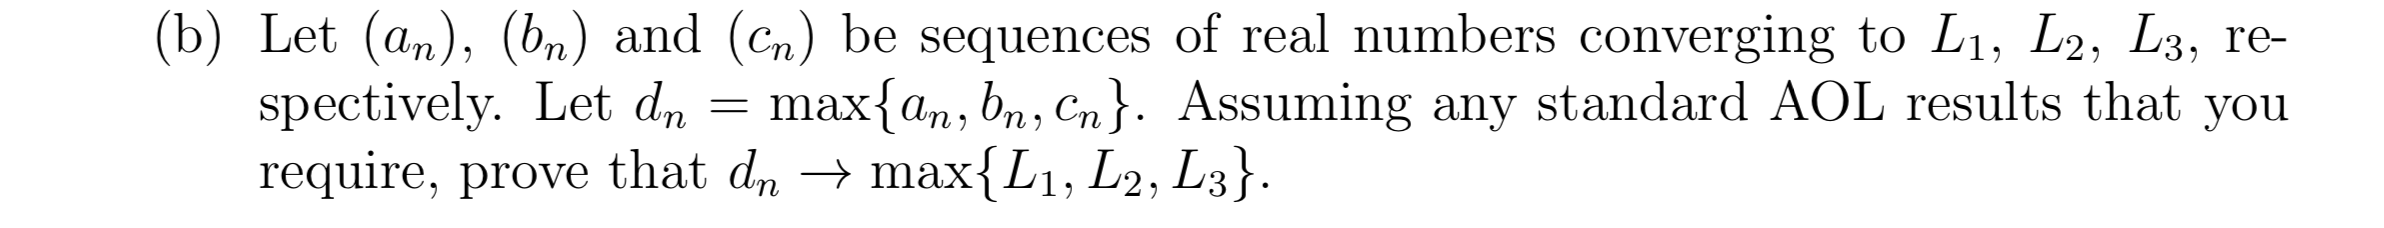
\includegraphics[width=400pt]{img/oxford-M2-analysis-I-4-4-b.png}
\end{mdframed}
\begin{proof}
  Let $(a_n)$, $(b_n)$, $(c_n)$ be real sequences with $(a_n) \to L_1$, $(b_n) \to L_2$,
  $(c_n) \to L_3$, and let $d_n = \max ~ \{a_n, b_n, c_n\}$.

  First suppose $L_1 = L_2 = L_3 = L$. Fix $\epsilon > 0$. Put $N = \max\{N_1, N_2, N_3\}$ where
  $N_1$, $N_2$, $N_3$ ``work'' for $(a_n)$, $(b_n)$, $(c_n)$ respectively, for this choice of
  $\epsilon$. Then $|d_n - L| < \epsilon$ for $n \geq N$, so $d_n \to L = \max\{L_1, L_2, L_3\}$.

  Finally, WLOG, suppose $L_1 > L_2 \geq L_3$. Let $\epsilon = L_1 - L_2$. Put
  $N = \max\{N_1, N_2, N_3\}$ where $N_1, N_2, N_3$ ``work'' for $(a_n), (b_n), (c_n)$
  respectively, for this choice of $\epsilon$. Then $a_n > b_n$ and $a_n > c_n$ for $n \geq
  N$. Therefore $d_n = a_n$ for $n \geq N$. Therefore $d_n \to L_1 = \max\{L_1, L_2, L_3\}$.

  \red{Right? But why does the question suggest AOL is needed?}
\end{proof}


\newpage
\subsection{}
\begin{mdframed}
  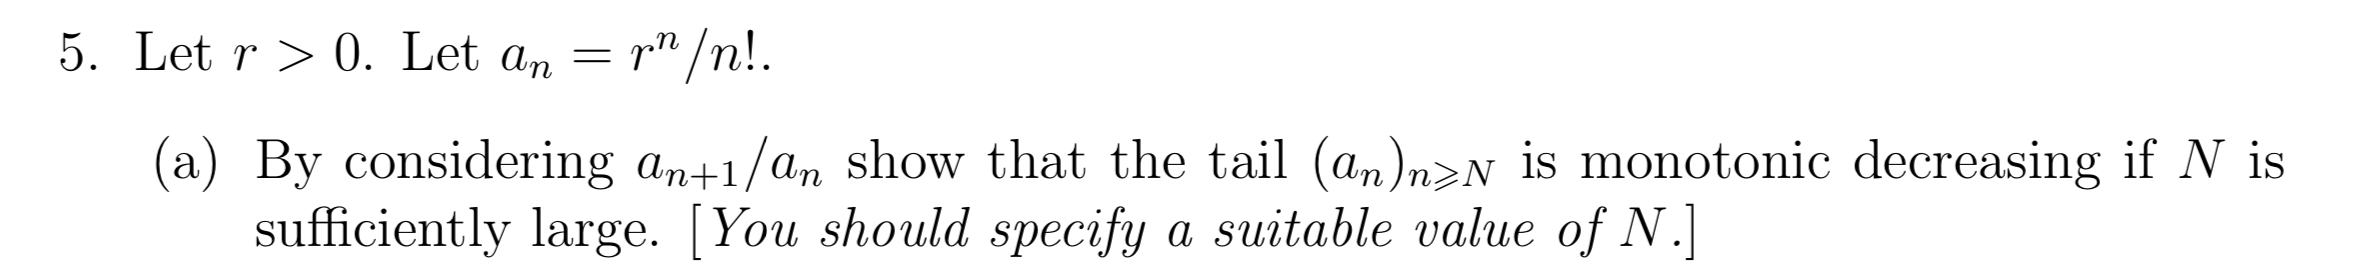
\includegraphics[width=400pt]{img/oxford-M2-analysis-I-4-5-a.png}
\end{mdframed}

\begin{proof}
  Let $r > 0$ and let $a_n = \frac{r^n}{n!}$. Then
  \begin{align*}
    \frac{a_{n+1}}{a_n} = \frac{r^{n+1}}{(n+1)!}\frac{n!}{r^n} = \frac{r}{n+1}.
  \end{align*}
  Therefore $(a_n)_{n \geq N}$ is monotonic decreasing for $N = \ceil{r}$.
\end{proof}

\begin{mdframed}
  
\includegraphics[width=400pt]{img/oxford-M2-analysis-I-4-5-b.png}
\end{mdframed}

\begin{proof}
  Note that $a_n > 0$. Since $(a_n)$ is bounded below by zero and the tail $(a_n)_{n \geq N}$ is
  monotonic decreasing for $N = \ceil{r}$, we have that $a_n$ converges to a limit $L > 0$ by the
  Monotonic Sequence Theorem.
\end{proof}

\begin{claim*}
  $a_n \to 0$.
\end{claim*}

\begin{proof}
  If $r \leq 1$ then $a_n \leq \frac{1}{n!} \to 0$.

  So let $r > 1$. Note that for $n > r$
  \begin{align*}
    a_n
    = \prod_{k=1}^{n}\frac{r}{k}
    = \(\prod_{k=1}^{\ceil{r} - 1}\frac{r}{k}\)\(\prod_{k=\ceil{r}}^n\frac{r}{k}\).
  \end{align*}

  The first factor is a product of terms each of which is greater than 1, and we have
  \begin{align*}
    \(\prod_{k=1}^{\ceil{r} - 1}\frac{r}{k}\) < r^{\ceil{r} - 1}.
  \end{align*}
  The second factor is a product of terms each of which is not greater than 1, and we have
  \begin{align*}
    \(\prod_{k=\ceil{r}}^n\frac{r}{k}\) < \(\frac{r}{\ceil{r}}\)^{n - \ceil{r} + 1}.
  \end{align*}
  \red{What about if $r = \ceil{r}$?}

  Therefore
  \begin{align*}
    a_n
    < r^{\ceil{r} - 1} \(\frac{r}{\ceil{r}}\)^{n - \ceil{r} + 1}
    = \(\frac{r}{\ceil{r}}\)^n\ceil{r}^{\ceil{r} - 1}
  \end{align*}

  \begin{mdframed}
    Scratch work:
    \begin{align*}
      \(\frac{r}{\ceil{r}}\)^n\ceil{r}^{\ceil{r} - 1} &< \epsilon\\
      \(\frac{r}{\ceil{r}}\)^n &< \epsilon \ceil{r}^{1 - \ceil{r}}\\
      n\log \frac{r}{\ceil{r}} &< \log \epsilon + (1 - \ceil{r})\ceil{r}\\
      n                        &> \frac{\log \epsilon + (1 - \ceil{r})\ceil{r}}
                                 {\log r - \log \ceil{r}}.
    \end{align*}
  \end{mdframed}

  Fix $\epsilon > 0$. Let
  $N = \Bigceil{\frac{\log \epsilon + (1 - \ceil{r})\log \ceil{r}} {\log r - \log \ceil{r}}}$.
  Then $a_n < \epsilon$ for $n \geq N$. Therefore $a_n \to 0$.
\end{proof}


\newpage
\subsection{}
\begin{mdframed}
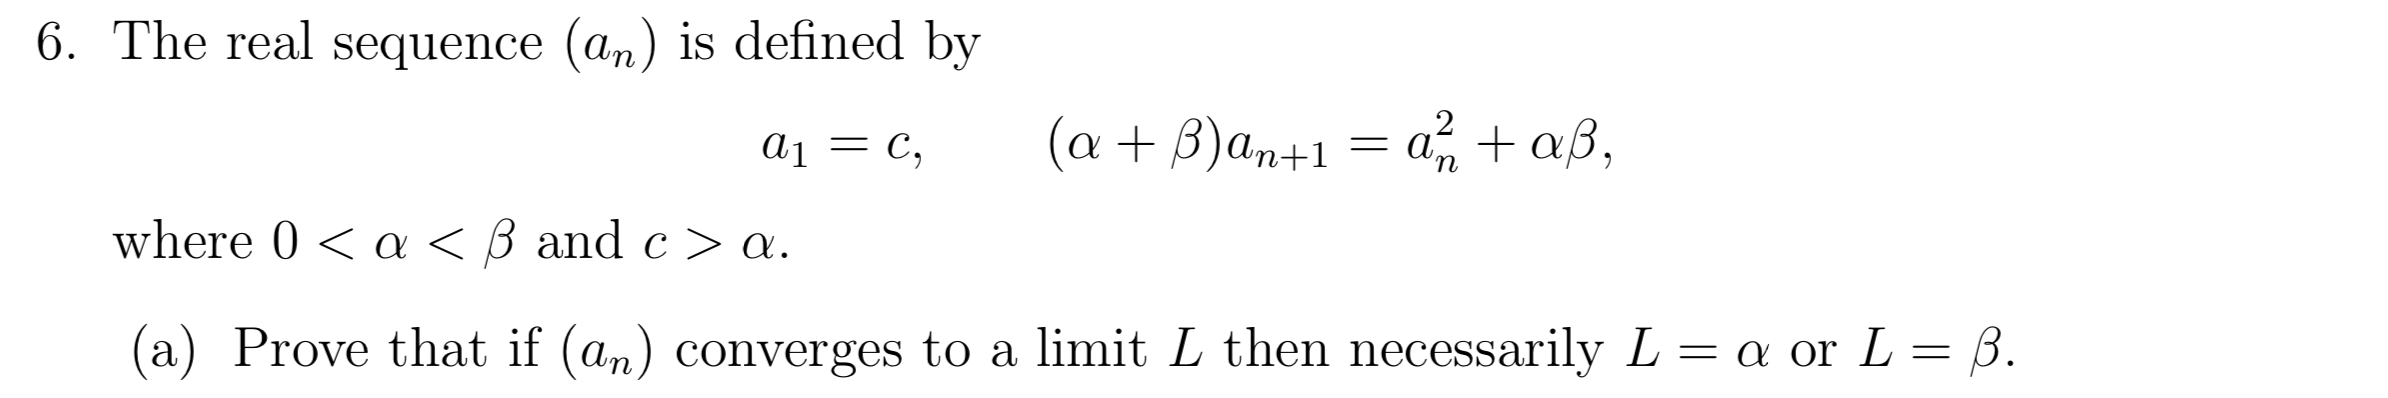
\includegraphics[width=400pt]{img/oxford-M2-analysis-I-4-6-a.png}
\end{mdframed}

\begin{proof}
  Let the real sequence $(a_n)$ be defined by
  \begin{align*}
    a_1 = c,  ~~~~~~~ (\alpha + \beta)a_{n+1} = a_n^2 + \alpha\beta.
  \end{align*}
  Assume $a_n \to L$. Then after taking limits of both sides as $n \to \infty$
  \begin{align*}
    L^2 - (\alpha + \beta)L + \alpha\beta = (L - \alpha)(L - \beta) = 0,
  \end{align*}
  therefore $L = \alpha$ or $L = \beta$.
\end{proof}

\begin{mdframed}
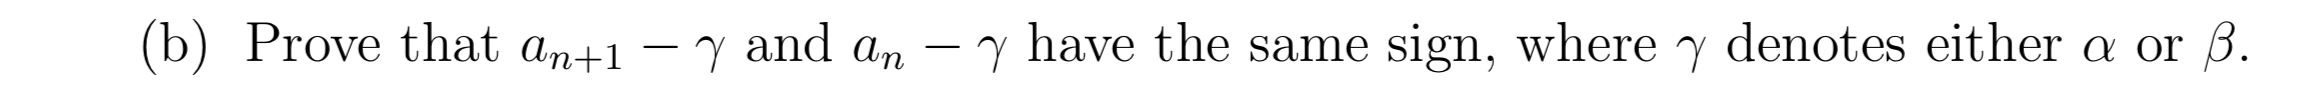
\includegraphics[width=400pt]{img/oxford-M2-analysis-I-4-6-b.png}
\end{mdframed}

\begin{proof}
  Consider
  \begin{align*}
    (a_{n+1} - \gamma)(a_n - \gamma) = \frac{}{}
  \end{align*}

  Suppose $a_n < \alpha$. Then
  \begin{align*}
    a_{n+1} - \alpha = \frac{\alpha a_n^2 + \alpha^2\beta - \alpha(\alpha + )}{\alpha + \beta} =
  \end{align*}
\end{proof}

\begin{mdframed}
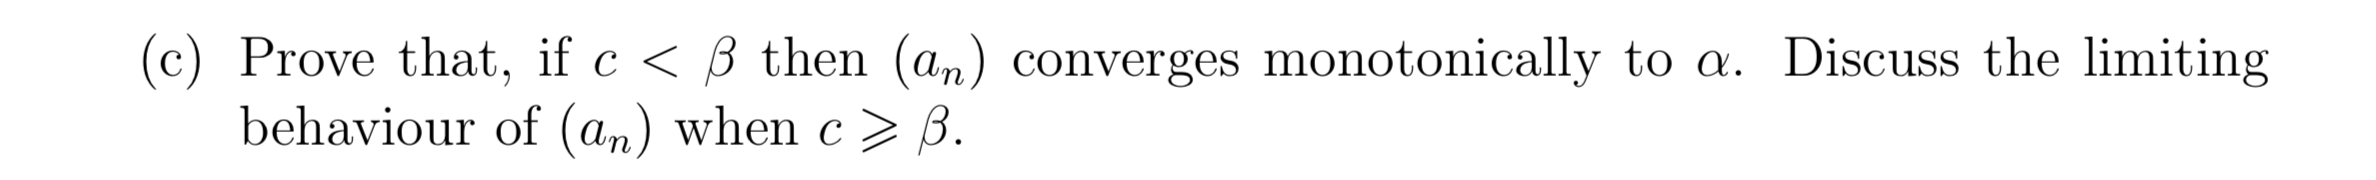
\includegraphics[width=400pt]{img/oxford-M2-analysis-I-4-6-c.png}
\end{mdframed}
\begin{mdframed}
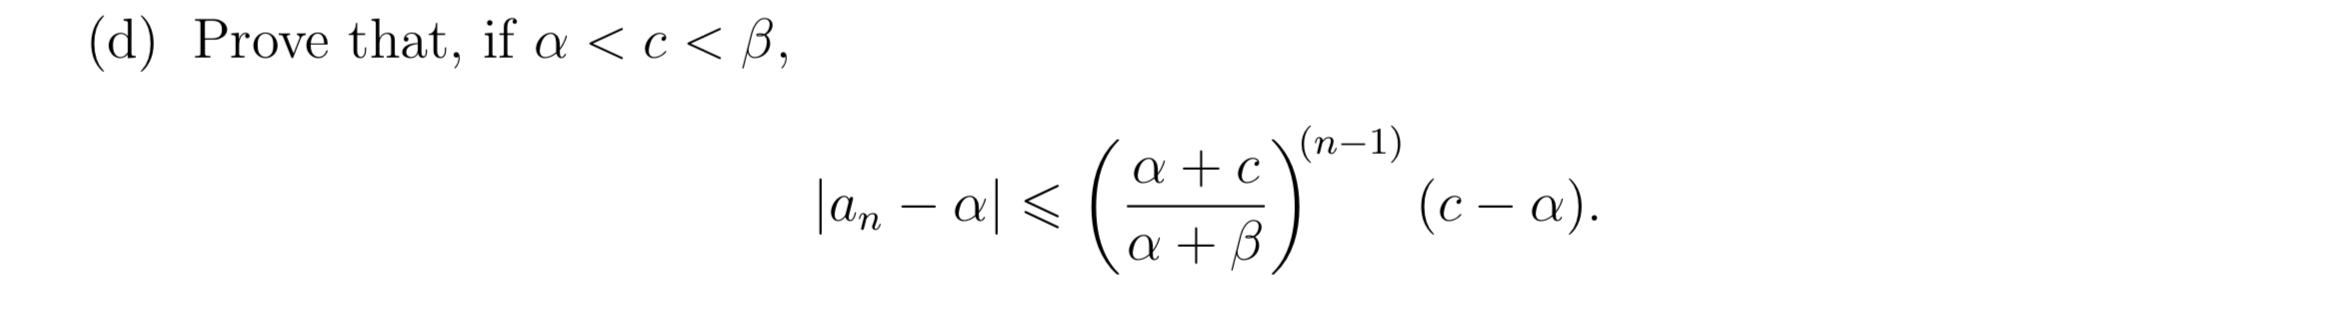
\includegraphics[width=400pt]{img/oxford-M2-analysis-I-4-6-d.png}
\end{mdframed}

\newpage
\subsection{}
\begin{mdframed}
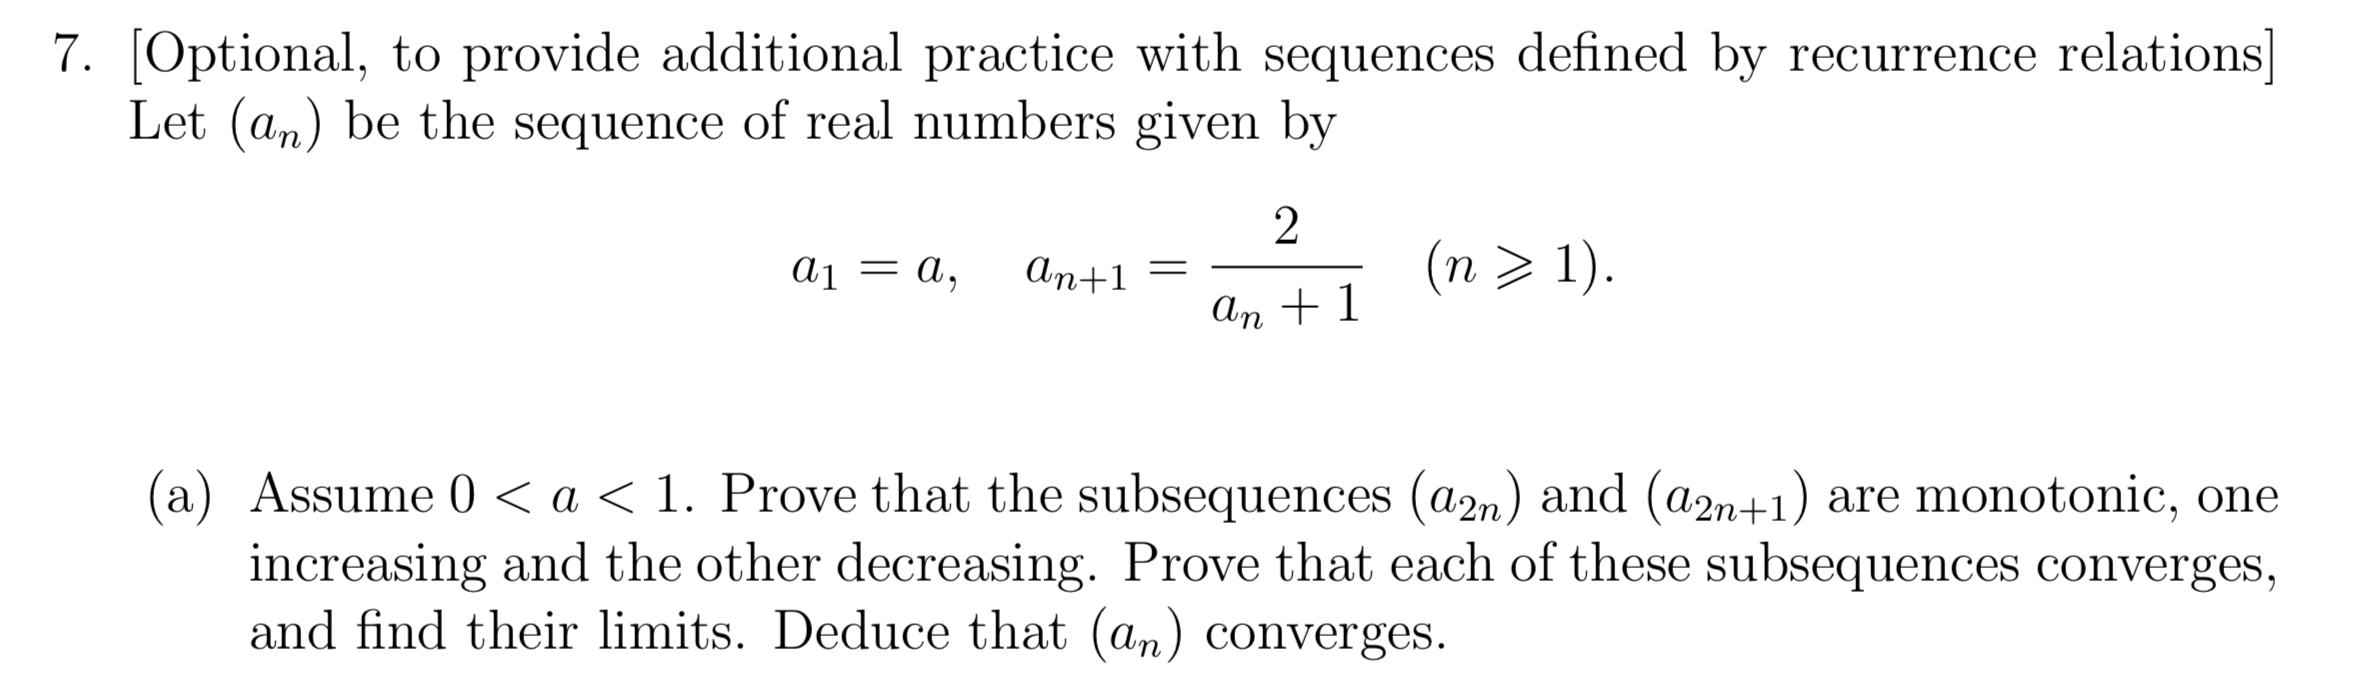
\includegraphics[width=400pt]{img/oxford-M2-analysis-I-4-7-a.png}
\end{mdframed}
\begin{mdframed}
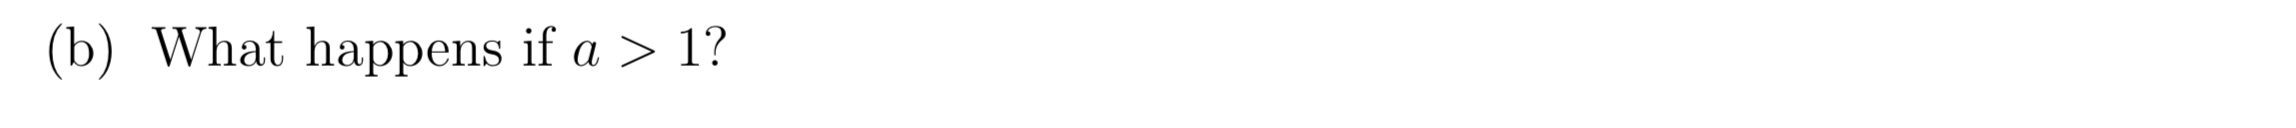
\includegraphics[width=400pt]{img/oxford-M2-analysis-I-4-7-b.png}
\end{mdframed}

\newpage
\subsection{}
\begin{mdframed}
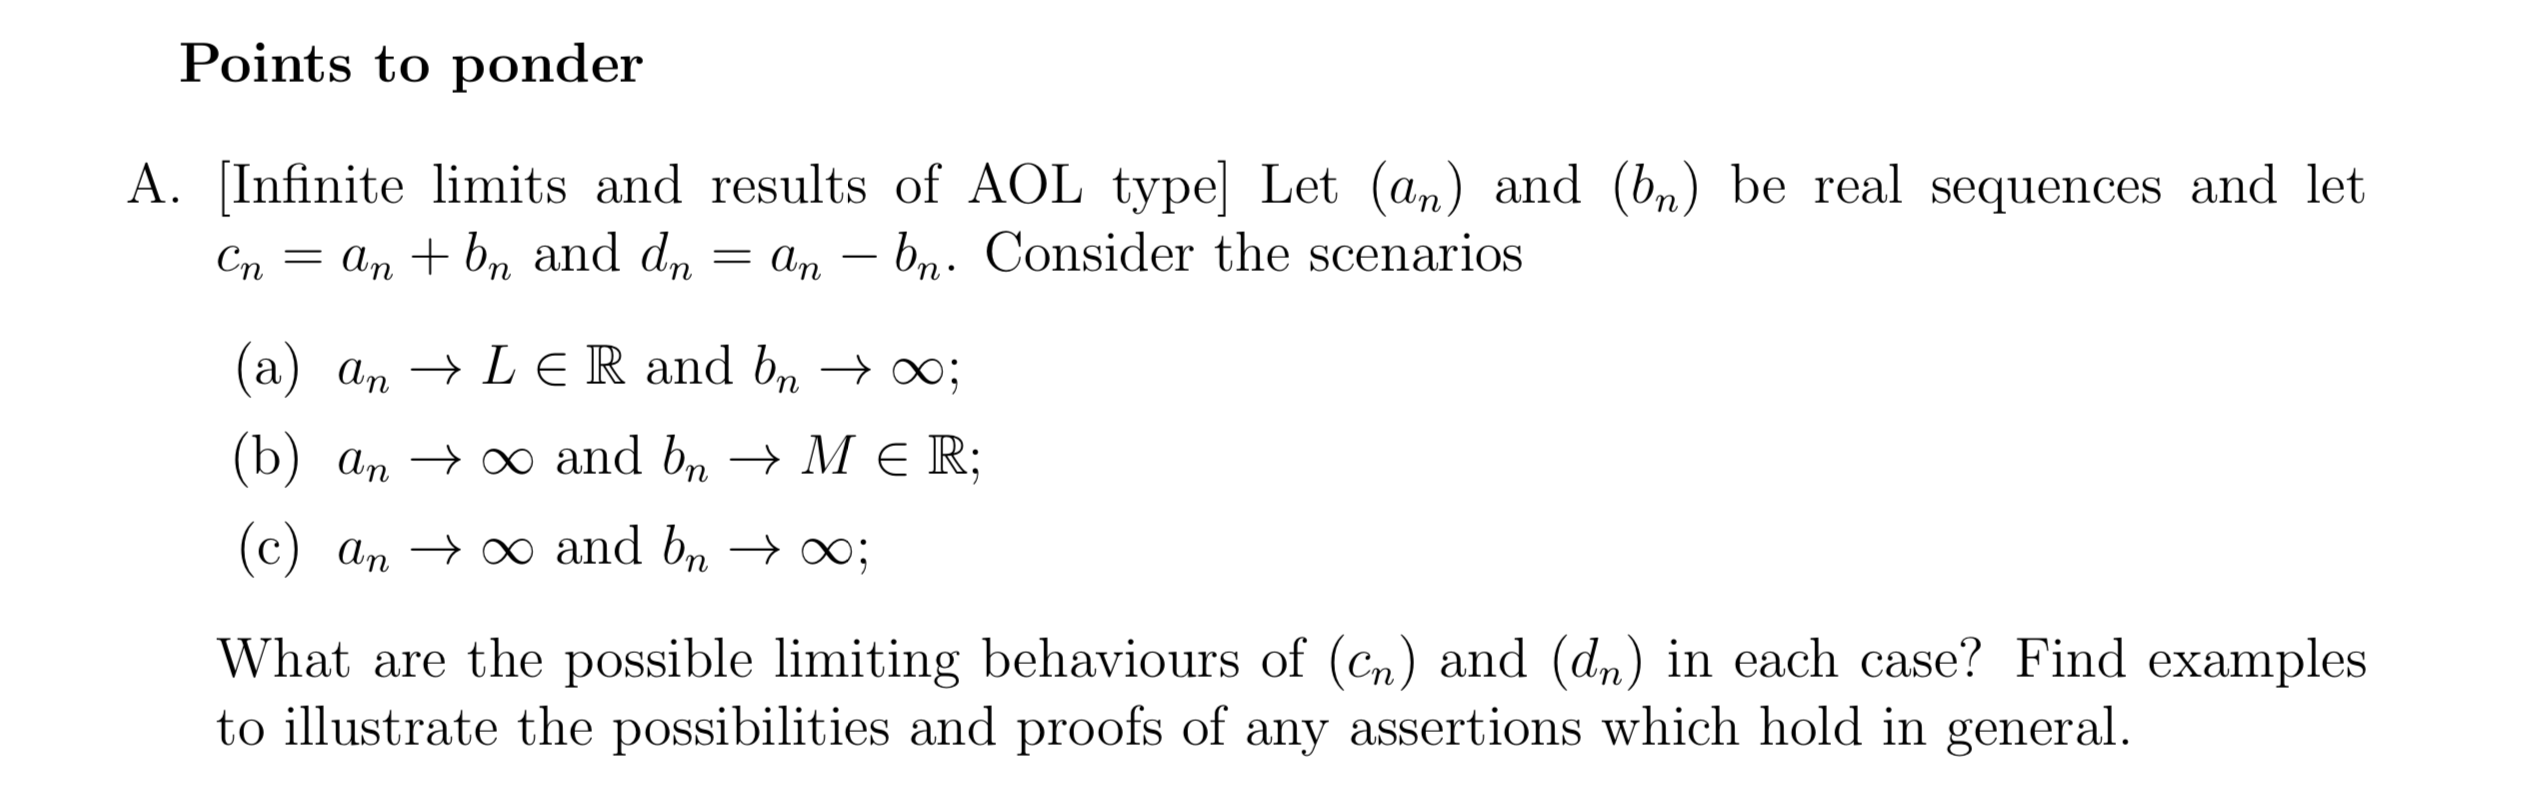
\includegraphics[width=400pt]{img/oxford-M2-analysis-I-extra-A.png}
\end{mdframed}
\begin{mdframed}
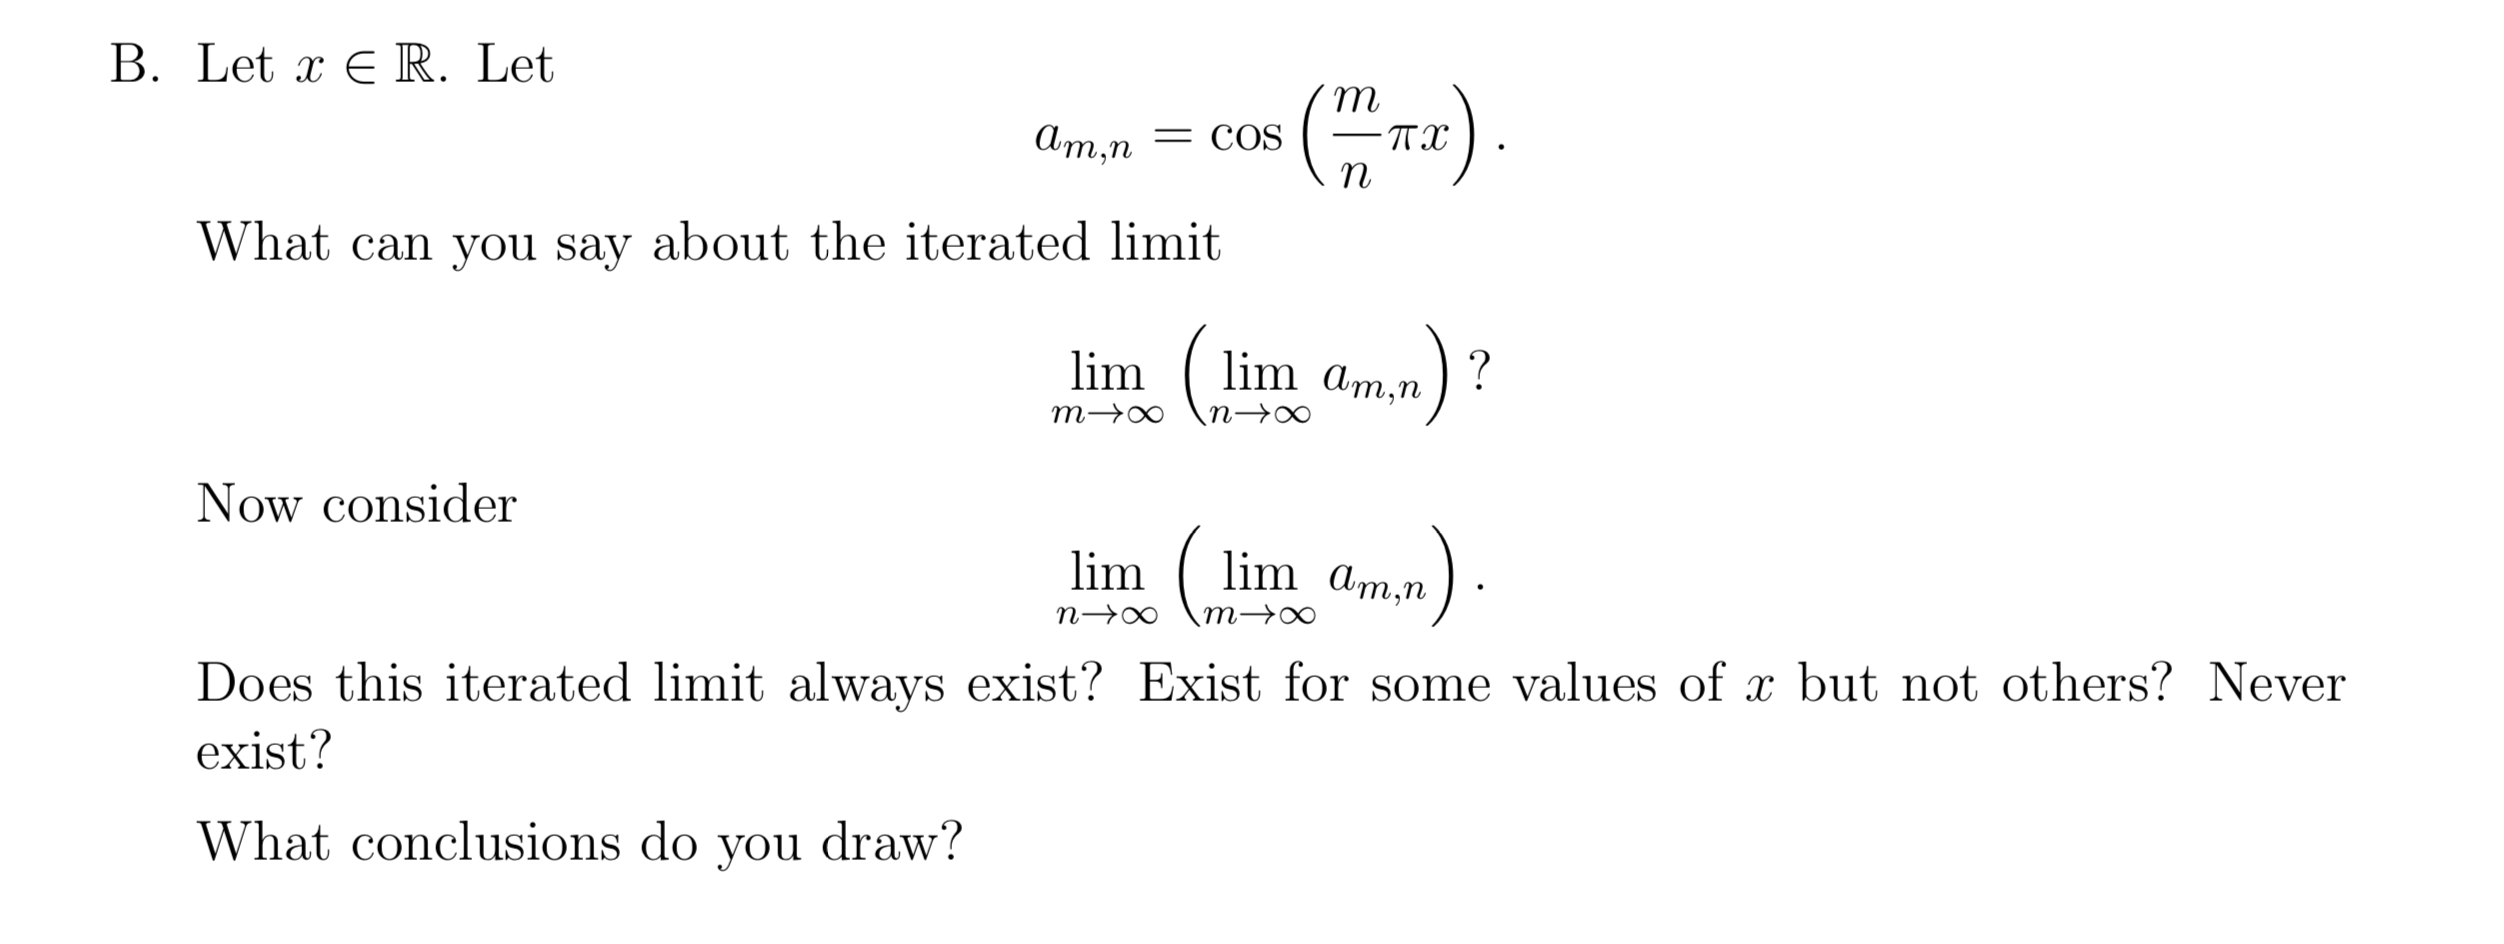
\includegraphics[width=400pt]{img/oxford-M2-analysis-I-extra-B.png}
\end{mdframed}

\section{Sheet 5}

\newpage
\subsection{}

\begin{mdframed}
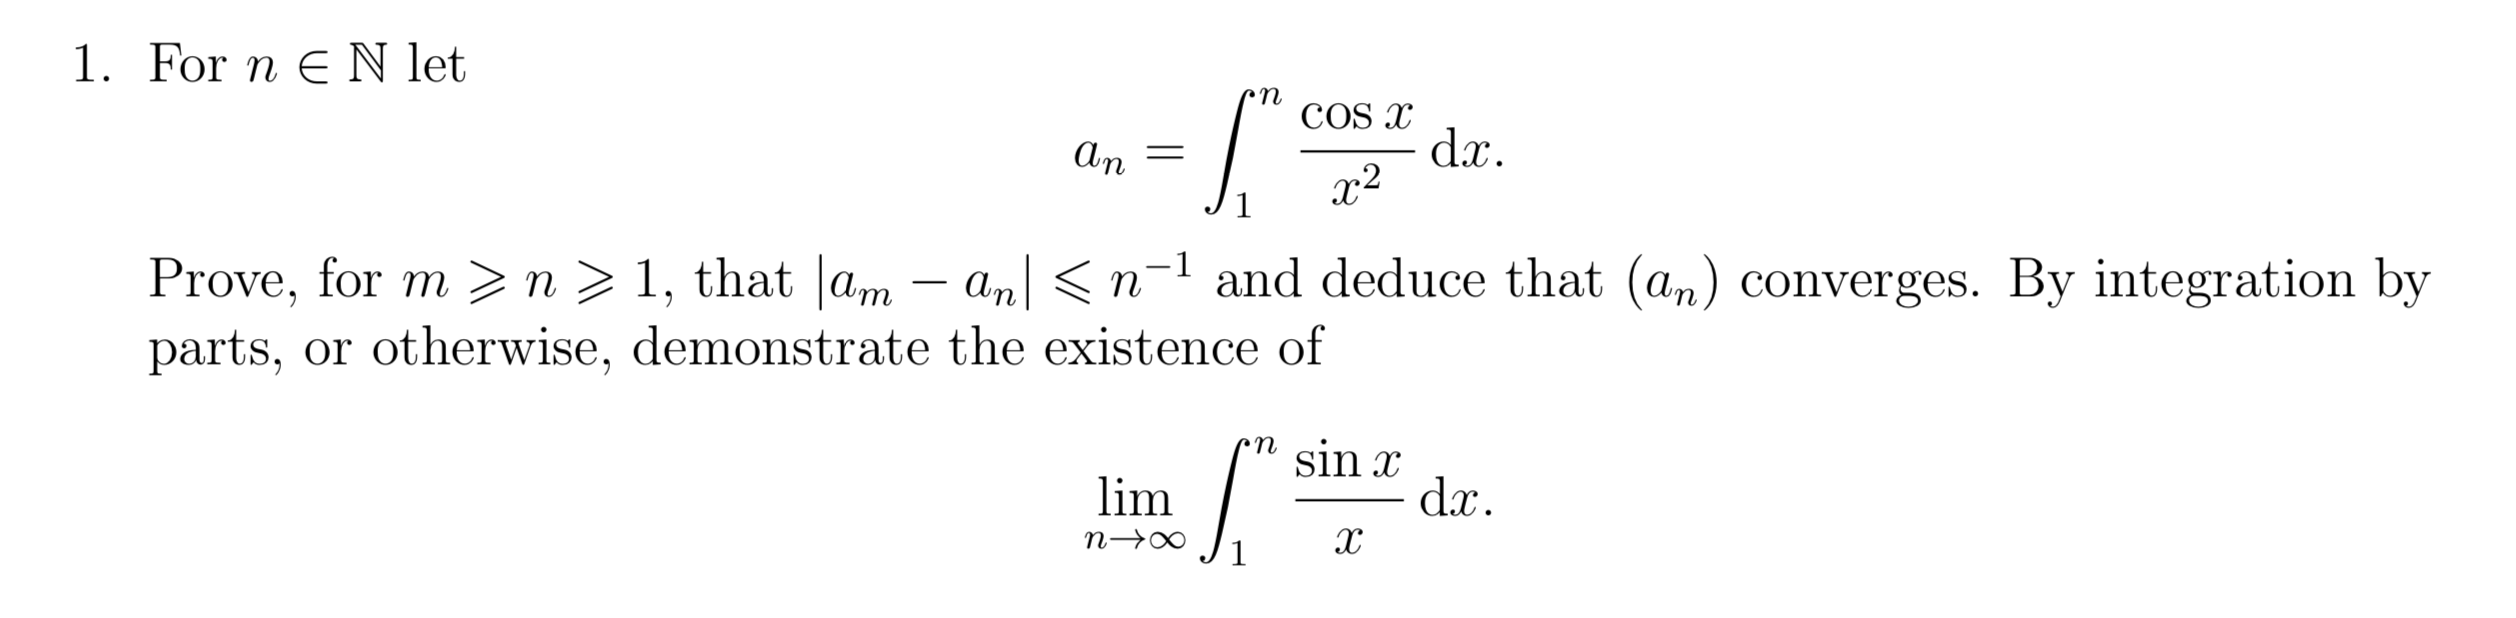
\includegraphics[width=400pt]{img/analysis--oxford-M2-I-5-1.png}
\end{mdframed}

\begin{proof}
  \begin{align*}
    |a_m - a_n| &=    \Big| \int_1^m \frac{\cos x}{x^2} \dx - \int_1^n \frac{\cos x}{x^2} \dx \Big|\\
                &=    \Big| \int_n^m \frac{\cos x}{x^2} \dx \Big|\\
                &\leq \int_n^m \Big| \frac{\cos x}{x^2} \Big| \dx \\
                &\leq \int_n^m \frac{1}{x^2} \dx \\
                &= \frac{1}{n} - \frac{1}{m}
                < \frac{1}{n}. ~~~~\text{\red{why does question give $\leq$}?}
  \end{align*}
\end{proof}
\begin{claim*}
  $(a_n)$ converges.
\end{claim*}
\begin{proof}
  Note that $a_1 = 0$ and $a_n = \sum_{k=1}^n (a_{k} - a_{k-1})$ for $n \geq 2$.

  The series $\sum_{k=1}^n (a_{k} - a_{k-1})$ converges absolutely... confused.

  Note that $a_n = \sum_{k=1}^n b_k$, where
  \begin{align*}
    b_k =
    \begin{cases}
      0,     ~~~~~~~~~~~~~~&k = 1\\
      \int_{k-1}^k \frac{\cos x}{x^2} \dx = a_{k} - a_{k-1},   ~~~~~~~&k \geq 2.
    \end{cases}
  \end{align*}
  Thus $(a_n)$ is a sequence of partial sums, which converges

  Note that $(a_n)$ is a sequence of partial sums. To see this, define
  \begin{align*}
    b_n =
    \begin{cases}
      0,     ~~~~~~~&n = 1\\
      a_n - a_{n-1}  &n \geq 2,
    \end{cases}
  \end{align*}
  and observe that $a_n = \sum_{k=1}^n b_k = 0 + (a_2 - 0) + (a_3 - a_2) + \ldots + (a_n - a_{n - 1})$.

\end{proof}

\newpage
\subsection{}
\begin{mdframed}
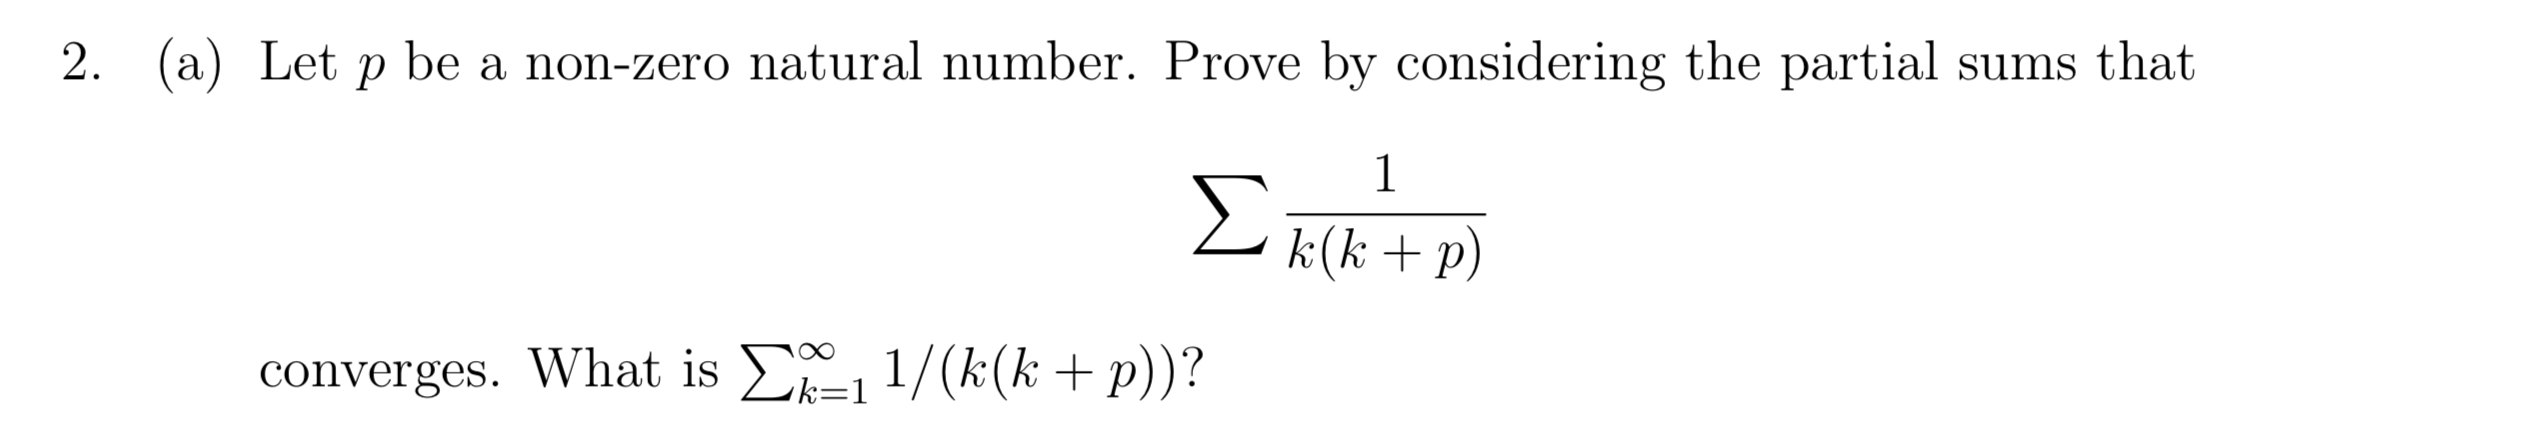
\includegraphics[width=400pt]{img/analysis--oxford-M2-I-5-2-a.png}
\end{mdframed}

\begin{claim*}
  $\sum \frac{1}{k(k+p)}$ converges.
\end{claim*}

\begin{proof}
  Let $p \in \N^+$ and define
  \begin{align*}
    a_k &= \frac{1}{k(k + p)}\\
    b_k &= \frac{1}{k^2}.
  \end{align*}
  Note that $\sum b_k$ converges and that $0 < a_k < b_k$. Therefore $\sum a_k$ converges.
\end{proof}

\newpage
\begin{claim*}
  $\sum_{k=1}^\infty \frac{1}{k(k+p)} = \sum_{k=1}^p\frac{1}{pk}$.
\end{claim*}

\begin{mdframed}
  Partial fractions:
\begin{align*}
  \frac{1}{k(k+p)} &= \frac{A}{k} + \frac{B}{k + p}\\
  (A + B)k + Ap &= 1\\
  A &= \frac{1}{p}, B = \frac{-1}{p}
\end{align*}
\end{mdframed}

\begin{proof}
  \begin{align*}
    \sum_{k=1}^\infty \frac{1}{k(k+p)} &= \sum_{k=1}^\infty \frac{1}{pk} - \frac{1}{p(k + p)}\\
                                       &= \sum_{k=1}^\infty \frac{1}{pk} - \sum_{k=p+1}^\infty  \frac{1}{pk}\\
                                       &= \sum_{k=1}^p\frac{1}{pk}.
  \end{align*}
\end{proof}

\begin{minted}{python3}
  def approx(p, n):
      return sum((1 / (k * (k + p))) for k in range(1, n + 1))

  def exact(p):
      return sum((1 / (p * k)) for k in range(1, p + 1))

  In [1]: exact(p=7)
  Out[1]: 0.3704081632653061

  In [2]: [approx(p=7, n=10**k) for k in [1, 2, 3, 7]]
  Out[2]:
  [0.2974675534549484,
   0.3607892203613656,
   0.36941214337664163,
   0.3704080632652916]
\end{minted}

\newpage
\begin{mdframed}
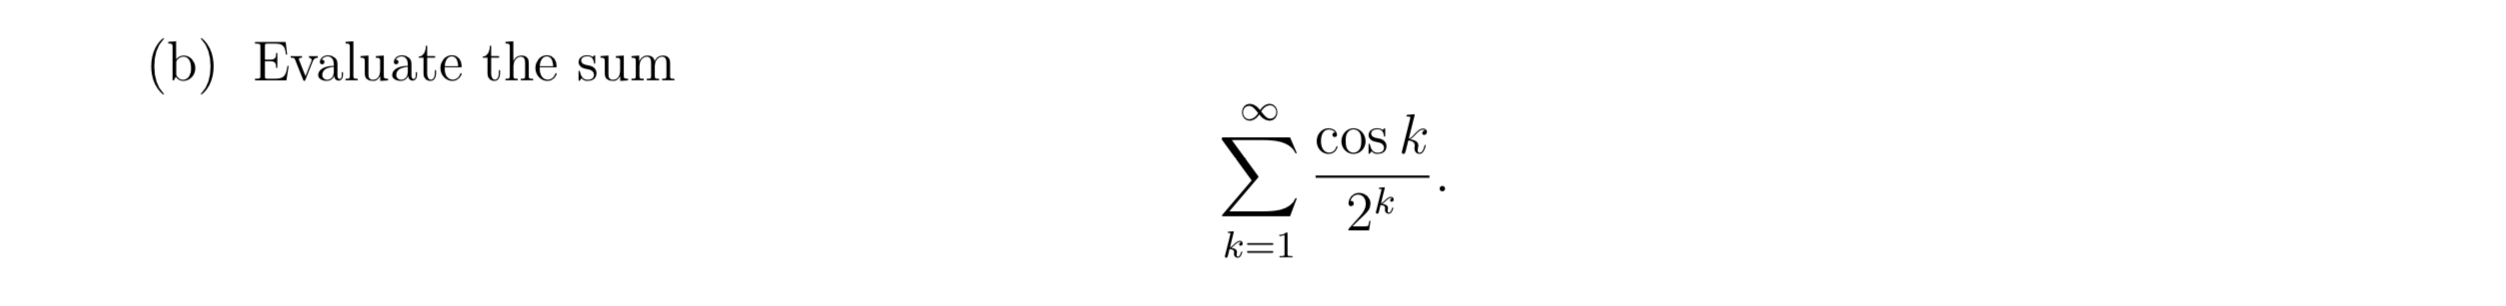
\includegraphics[width=400pt]{img/analysis--oxford-M2-I-5-2-b.png}
\end{mdframed}

\red{INCOMPLETE}

\begin{minted}{python3}
  In [19]: sum(cos(k) / 2**k for k in range(1, 10 + 1))
  Out[19]: 0.0281023042150256

  In [20]: sum(cos(k) / 2**k for k in range(1, 100 + 1))
  Out[20]: 0.028393995218935916

  In [21]: sum(cos(k) / 2**k for k in range(1, 1000 + 1))
  Out[21]: 0.028393995218935916
\end{minted}

\begin{proof}
  \begin{align*}
    \sum_{k=1}^\infty \frac{\cos k}{2^k} = \frac{\cos 1}{2^1} + \frac{\cos 2}{2^2} + \frac{\cos 3}{2^3} + \dots\\
  \end{align*}
\end{proof}

\newpage
\begin{mdframed}
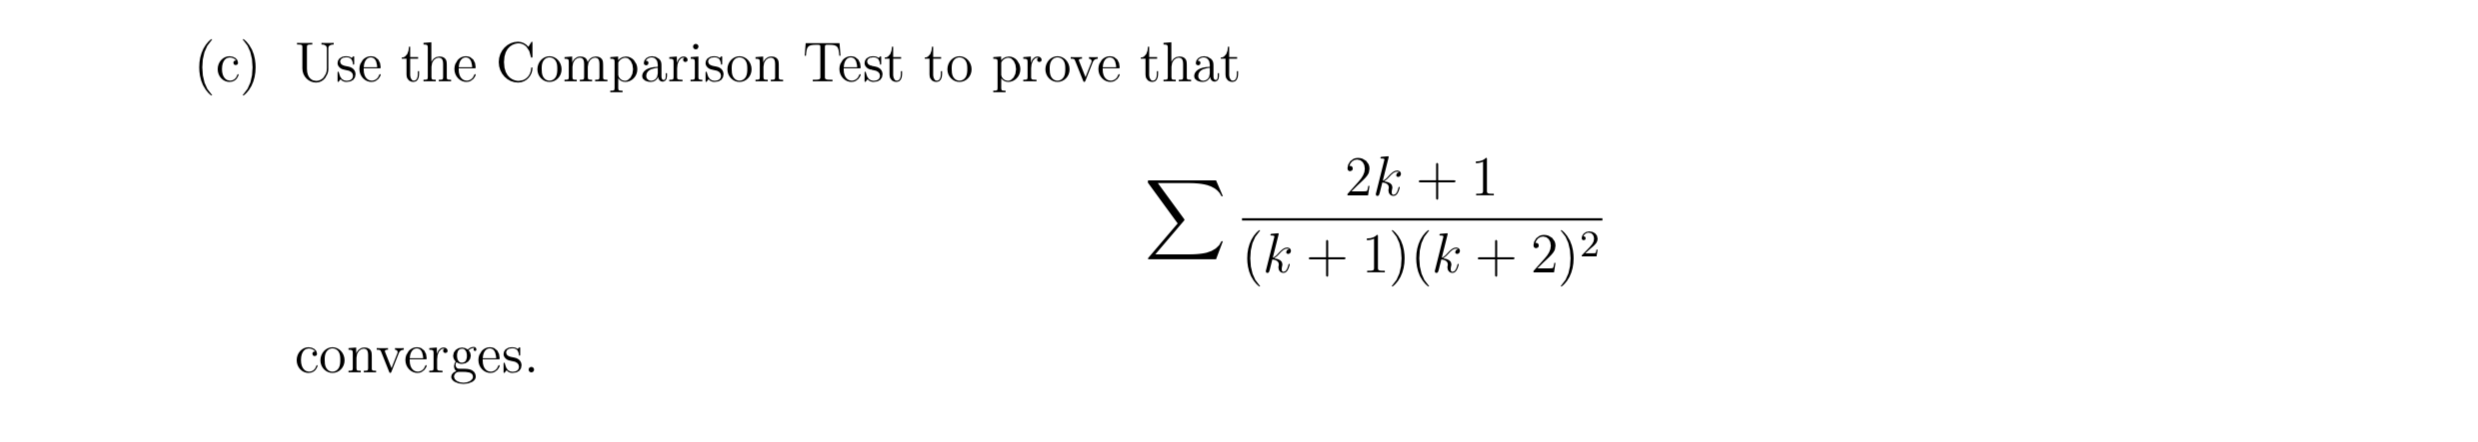
\includegraphics[width=400pt]{img/analysis--oxford-M2-I-5-2-c.png}
\end{mdframed}

\begin{proof}
  Define $a_k = \frac{2k + 1}{(k + 1)(k + 2)^2}$ and $b_k = \frac{1}{k(k + 1)}$. Note that
  \begin{align*}
    a_k
    &= \frac{2k}{(k + 2)^2(k + 1)} + \frac{1}{(k + 2)^2(k + 1)}\\
    &< \frac{2}{k(k + 1)} + \frac{1}{k(k + 1)}\\
    &= 3b_k
  \end{align*}
  We showed in part (a) that $\sum b_k$ converges. Therefore $\sum a_k$ converges.
\end{proof}

\newpage
\subsection{}
\begin{mdframed}
\includegraphics[width=400pt]{img/analysis--oxford-M2-I-5-3.png}
\end{mdframed}
\begin{claim*}
  $\Big|\sum\limits_{k=1}^\infty a_k\Big| \leq \sum\limits_{k=1}^\infty |a_k|$.
\end{claim*}

\begin{proof}
  Let $(a_n)$ be a complex sequence and assume that $\sum_{k=1}^n |a_k|$ converges.

  Define
  \begin{align*}
    s_n = a_1 + \ldots + a_n ~~~~~~~\text{and}~~~~~~~ S_n = |a_1| + \ldots + |a_n|.
  \end{align*}

  Consider the sequences $(|s_n|)$ and $(S_n)$.

  Note that $|s_n| \leq S_n$ for all $n$ by the Triangle Law.

  Note also that $(S_n)$ converges, say to $L$, by hypothesis, and therefore that $(|s_n|)$
  converges, say to $M$.

  We have $L \leq M$ by Preservation of Weak Inequalities.
\end{proof}

\begin{mdframed}
  \includegraphics[width=400pt]{img/analysis--oxford-M2-I-preservation-weak-inequalities.png}
\end{mdframed}



\newpage
\subsection{}
\begin{mdframed}
\includegraphics[width=400pt]{img/analysis--oxford-M2-I-5-4-a.png}
\end{mdframed}

\begin{proof}
  Let $s_n = \sum_{k=0}^n \frac{1}{k!}$.

  \red{INCOMPLETE}

  Note that $s_n > \sum_{k=0}^n \frac{1}{n^k} = \frac{n}{n-1} \to 1$, but that's not helpful.
\end{proof}

\begin{mdframed}
\includegraphics[width=400pt]{img/analysis--oxford-M2-I-5-4-b.png}
\end{mdframed}

\begin{proof}

\end{proof}
\newpage
\subsection{}
\begin{mdframed}
\includegraphics[width=400pt]{img/analysis--oxford-M2-I-5-5.png}
\end{mdframed}
\begin{proof}
  \red{INCOMPLETE}
  \begin{align*}
    \(1 - \frac{1}{n}\)^n
    &= \sum_{k=0}^n(-1)^k\frac{{n \choose k}}{n^k}\\
    &= \sum_{k=0}^n(-1)^k\frac{n(n-1)\cdots(n-k+1)}{k!n^k}\\
%    &= \sum_{k=0}^n\Big((-1)^k\frac{1}{k!} + O\(\frac{1}{n}\)\Big)\\
    &= 1 - \frac{n}{n} + \frac{n(n-1)}{2\cdot n^2} - \frac{n(n-1)(n-2)}{3\cdot 2\cdot n^3} + \ldots + (-1)^n\frac{1}{n^n}\\ % \frac{n(n-1)(n-2)(n-3)}{4\cdot 3\cdot 2\cdot n^4} -
    &= \frac{n - 1}{2!n} - \frac{(n-1)(n-2)}{3!n^2} + \ldots + (-1)^n\\ % \frac{(n-1)(n-2)(n-3)}{4!n^3} -
    &= \frac{1 -\frac{1}{n}}{2!} - \frac{1 - 3\frac{1}{n} + 3\frac{1}{n^2}}{3!} + \ldots\\
  \end{align*}
\end{proof}

\newpage
\subsection{}
\begin{mdframed}
\includegraphics[width=400pt]{img/analysis--oxford-M2-I-5-6-a.png}
\end{mdframed}

\begin{proof}
  Let $a_k = (\sqrt{k+1} - \sqrt{k})$. Note that:

  \begin{enumerate}[label=(\roman*)]
  \item $a_k = \frac{1}{\sqrt{k+1} + \sqrt{k}} > 0$.
  \item
    $a_k - a_{k+1} = \frac{1}{\sqrt{k+1} + \sqrt{k}} - \frac{1}{\sqrt{k+2} + \sqrt{k + 1}} >
    \frac{1}{2\sqrt{k+1}} - \frac{1}{2\sqrt{k+1}}$, by making the first term bigger and the second
    smaller. Therefore $a_{k+1} < a_k$.
  \item $0 < a_k < \frac{1}{\sqrt{k}}$. Fix $\epsilon > 0$ and note that
    $n \geq \ceil{\frac{1}{\epsilon^2}} + 1 \implies \frac{1}{\sqrt{n}} < \epsilon$. Therefore
    $\frac{1}{\sqrt{k}} \to 0$. Therefore $a_k \to 0$.
  \end{enumerate}
  Therefore $\sum (-1)^{k-1}a_k$ converges by the Alternating Series Test.
\end{proof}

\begin{mdframed}
\includegraphics[width=400pt]{img/analysis--oxford-M2-I-5-6-b.png}
\end{mdframed}



\newpage
\subsection{}
\begin{mdframed}
\includegraphics[width=400pt]{img/analysis--oxford-M2-I-5-7.png}
\end{mdframed}

\begin{proof}\hspace{0pt}
  \begin{enumerate}[label=(\alph*)]
  \item False. A counterexample is $a_k = \frac{1}{k^3}$ since then $k^2a_k = \frac{1}{k} \to 0$
    yet $\sum \frac{1}{k}$ is divergent.
  \item False. A counterexample is $a_k = (-1)^k\frac{1}{\sqrt{k}}$ since then $\sum a_k$ converges
    but $\sum a_k^2$ diverges.
  \item I think this is true. Proof? Suppose $\sum |a_k|$ converges to $L$...
  \item ?
  \end{enumerate}
\end{proof}

\newpage
\subsection{}
\begin{mdframed}
\includegraphics[width=400pt]{img/analysis--oxford-M2-I-5-8-a.png}
\end{mdframed}

\begin{mdframed}
\includegraphics[width=400pt]{img/analysis--oxford-M2-I-5-8-b.png}
\end{mdframed}

\end{document}